% abtex2-modelo-artigo.tex, v-1.9.2 laurocesar
% Copyright 2012-2014 by abnTeX2 group at http://abntex2.googlecode.com/ 
%

% ------------------------------------------------------------------------
% ------------------------------------------------------------------------
% abnTeX2: Modelo de Artigo Acadêmico em conformidade com
% ABNT NBR 6022:2003: Informação e documentação - Artigo em publicação 
% periódica científica impressa - Apresentação
% ------------------------------------------------------------------------
% ------------------------------------------------------------------------

\documentclass[
	% -- opções da classe memoir --
	article,			% indica que é um artigo acadêmico
	11pt,				% tamanho da fonte
	oneside,			% para impressão apenas no verso. Oposto a twoside
	a4paper,			% tamanho do papel. 
	% -- opções da classe abntex2 --
	%chapter=TITLE,		% títulos de capítulos convertidos em letras maiúsculas
	%section=TITLE,		% títulos de seções convertidos em letras maiúsculas
	%subsection=TITLE,	% títulos de subseções convertidos em letras maiúsculas
	%subsubsection=TITLE % títulos de subsubseções convertidos em letras maiúsculas
	% -- opções do pacote babel --
	english,			% idioma adicional para hifenização
	brazil,				% o último idioma é o principal do documento
	sumario=tradicional
	]{abntex2}


% ---
% PACOTES
% ---

% ---
% Pacotes fundamentais 
% ---
\usepackage{lmodern}			% Usa a fonte Latin Modern
\usepackage[T1]{fontenc}		% Selecao de codigos de fonte.
\usepackage[utf8]{inputenc}		% Codificacao do documento (conversão automática dos acentos)
\usepackage{indentfirst}		% Indenta o primeiro parágrafo de cada seção.
\usepackage{nomencl} 			% Lista de simbolos
\usepackage{color}				% Controle das cores
\usepackage{graphicx}			% Inclusão de gráficos
\usepackage{microtype} 			% para melhorias de justificação
% ---
		
% ---
% Pacotes adicionais, usados apenas no âmbito do Modelo Canônico do abnteX2
% ---
\usepackage{lipsum}				% para geração de dummy text
% ---
		
% ---
% Pacotes de citações
% ---
\usepackage[brazilian,hyperpageref]{backref}	 % Paginas com as citações na bibl
\usepackage[alf]{abntex2cite}	% Citações padrão ABNT
% ---

% ---
% Pacotes extras
% ---
\usepackage{amsmath}    % Pacote para matemática
\usepackage{float}      % Pacote para controle de formatação de imagens 
                        % e tabelas

% ---
% Configurações do pacote backref
% Usado sem a opção hyperpageref de backref
\renewcommand{\backrefpagesname}{Citado na(s) página(s):~}
% Texto padrão antes do número das páginas
\renewcommand{\backref}{}
% Define os textos da citação
\renewcommand*{\backrefalt}[4]{
	\ifcase #1 %
		Nenhuma citação no texto.%
	\or
		Citado na página #2.%
	\else
		Citado #1 vezes nas páginas #2.%
	\fi}%
% ---

% ---
% Informações de dados para CAPA e FOLHA DE ROSTO
% ---
\titulo{Problema 2: ... Rega Automatizada (Melhorias)!}
\autor{
    Cláudio Daniel Figueredo Peruna \thanks{danielperuna2012@gmail.com} 
    \and Paulo Gabriel da Rocha Costa Silva \thanks{paulogrcsilva@gmail.com}
    \and Paulo Henrique Dantas Barreto \thanks{rickdeuxvult@gmail.com}
}
\local{Feira de Santana - Bahia}
\data{2024}
% ---

% ---
% Configurações de aparência do PDF final

% alterando o aspecto da cor azul
\definecolor{blue}{RGB}{41,5,195}

% informações do PDF
\makeatletter
\hypersetup{
     	%pagebackref=true,
		pdftitle={\@title}, 
		pdfauthor={\@author},
    	pdfsubject={Modelo de artigo científico com abnTeX2},
	    pdfcreator={LaTeX with abnTeX2},
		pdfkeywords={abnt}{latex}{abntex}{abntex2}{atigo científico}, 
		colorlinks=true,       		% false: boxed links; true: colored links
    	linkcolor=blue,          	% color of internal links
    	citecolor=blue,        		% color of links to bibliography
    	filecolor=magenta,      		% color of file links
		urlcolor=blue,
		bookmarksdepth=4
}
\makeatother
% --- 

% ---
% compila o indice
% ---
\makeindex
% ---

% ---
% Altera as margens padrões
% ---
\setlrmarginsandblock{3cm}{3cm}{*}
\setulmarginsandblock{3cm}{3cm}{*}
\checkandfixthelayout
% ---

% --- 
% Espaçamentos entre linhas e parágrafos 
% --- 

% O tamanho do parágrafo é dado por:
\setlength{\parindent}{1.3cm}

% Controle do espaçamento entre um parágrafo e outro:
\setlength{\parskip}{0.2cm}  % tente também \onelineskip

% Espaçamento simples
\SingleSpacing

% ----
% Início do documento
% ----
\begin{document}

% Retira espaço extra obsoleto entre as frases.
\frenchspacing 

% ----------------------------------------------------------
% ELEMENTOS PRÉ-TEXTUAIS
% ----------------------------------------------------------

%---
%
% Se desejar escrever o artigo em duas colunas, descomente a linha abaixo
% e a linha com o texto ``FIM DE ARTIGO EM DUAS COLUNAS''.
% \twocolumn[    		% INICIO DE ARTIGO EM DUAS COLUNAS
%
%---
% página de titulo
\maketitle

% resumo em português
\begin{resumoumacoluna}
Este estudo apresenta a evolução de um sistema automatizado de irrigação, inicialmente proposto, com a implementação de um circuito aprimorado. O novo design incorpora funcionalidades avançadas, incluindo um cronômetro e uma interface de visualização aprimorada das informações do sistema. As ferramentas de desenvolvimento \textit{Verilog} e \textit{Quartus} foram empregadas para a implementação na placa \textit{CPLD MAX II}. Os resultados demonstram a eficácia do uso de recursos como contadores sincronos e assincronos, \textit{flip-flops}, \textit{latches} e manipulação de \textit{clocks}, evidenciando o potencial do sistema para otimizar processos de irrigação.
 
 \vspace{\onelineskip}
 
 \noindent
 \textbf{Palavras-chaves}: irrigação automatizada. circuitos digitais. verilog. quartus. CPLD MAX II. sistemas digitais. contadores síncronos. contadores assíncronos. flip-flops. latches. manipulação de clocks. automação agrícola. otimização de processos.
\end{resumoumacoluna}

% ]  				% FIM DE ARTIGO EM DUAS COLUNAS
% ---

% ----------------------------------------------------------
% ELEMENTOS TEXTUAIS
% ----------------------------------------------------------
\textual

% ----------------------------------------------------------
% Introdução
% ----------------------------------------------------------
\section*{Introdução}

A evolução tecnológica é um processo contínuo e inexorável. Como observa Bill Gates, "Nós sempre superestimamos as mudanças que ocorrerão nos próximos dois anos e subestimamos as mudanças que ocorrerão na próxima década. Não se deixe levar pela inércia. Este é um momento emocionante"  \cite{gates1995}. Este dinamismo exige que inovações sejam constantemente atualizadas e melhoradas para acompanhar as demandas emergentes. No contexto da agricultura, a eficiência e a sustentabilidade dos processos são fundamentais. 

Com isso em mente, este estudo visa aprimorar um sistema automatizado de irrigação previamente desenvolvido, incorporando um novo circuito com funcionalidades avançadas. Este avanço foi implementado utilizando as ferramentas de desenvolvimento \textit{Verilog} e \textit{Quartus} na plataforma \textit{CPLD MAX II}. As melhorias incluem a adição de um cronômetro e uma interface de visualização mais sofisticada, com as imagens sendo mostradas na matriz de LEDs da placa, e não mais no seu \textit{display} de 7 segmentos. Dessa forma, esses enriquecimentos do projeto atendem melhor às necessidades dos usuários e otimizam o uso dos recursos hídricos.


% ----------------------------------------------------------
% Seção de Metodologia
% ----------------------------------------------------------

\section{Metodologia}

A metodologia adotada seguiu uma sequência de etapas bem definidas, conforme descrito a seguir:

\begin{enumerate}
\item Definição da Visão Geral e Diagramação de Alto Nível do Projeto: Inicialmente, elaborou-se uma visão abrangente do projeto, seguida pela criação de diagramas de alto nível, os quais delinearam as interações e os principais componentes do sistema.

\item Listagem dos Módulos Necessários: Posteriormente, realizou-se a identificação e a especificação detalhada dos módulos funcionais para a consecução do projeto.

\item Escolha das Ferramentas Utilizadas: Em seguida, selecionaram-se as ferramentas mais adequadas para o desenvolvimento do projeto, com base em critérios técnicos específicos.

\item Implementação da Projeção Utilizando \textit{Verilog}: Por fim, procedeu-se à implementação do projeto, empregando a linguagem de descrição de hardware \textit{Verilog}, assegurando a conformidade com as especificações estabelecidas nas etapas anteriores.
    
\end{enumerate}



\subsection{Ferramentas Utilizadas}

No contexto do presente estudo, as metodologias e ferramentas empregadas são uma continuação das práticas adotadas no projeto anterior, com a intenção de aprimorar a eficiência e a integração do desenvolvimento de sistemas digitais. A placa de desenvolvimento eletrônica escolhida para este projeto é a \textit{EPM240T100C5N}, pertencente à família \textit{MAX II}, que foi selecionada por suas capacidades robustas e compatibilidade com o ambiente de desenvolvimento.

O código que descreve o circuito foi escrito utilizando o \textit{Verilog HDL}, uma linguagem de descrição de hardware amplamente utilizada na indústria, conhecida por sua capacidade de modelar circuitos digitais. A compilação do código foi realizada no \textit{Quartus II}, uma ferramenta de design de circuitos integrados da \textit{Intel}, versão 20, que oferece uma plataforma poderosa para a implementação de designs em \textit{hardware}.

Para o desenvolvimento da descrição de hardware, foi preferido o uso da IDE do \textit{Visual Studio Code}, uma ferramenta moderna e flexível que proporciona uma experiência de desenvolvimento integrado otimizada. Mesmo que o código seja compilado no \textit{Quartus II}, o \textit{Visual Studio Code} foi utilizado para sua escrita e edição, aproveitando-se das funcionalidades avançadas da IDE para melhorar a produtividade do desenvolvedor.

A transferência e atualização do repositório contendo o código foram facilitadas pelo uso do \textit{Git} e do serviço \textit{GitHub}, que permitem uma colaboração eficiente entre diferentes máquinas, garantindo a integridade e a continuidade do projeto.

\subsection{Escrita do código e Documentação}

Para garantir que o código atingisse o máximo nível de legibilidade e intuitividade, adotou-se o uso de variáveis autoexplicativas e de nomenclatura clara. Além disso, incorporaram-se comentários detalhados em todas as seções do código, o que não apenas facilita o entendimento dos processos implementados, mas também elimina ambiguidade. Partes do código consideradas redundantes foram removidas. Adicionalmente, foram inseridas tabelas e informações relevantes na forma de comentários, proporcionando um referencial imediato que enriquece a compreensão contextual do código por parte dos leitores. Essa abordagem sistemática visa a otimização do código, assegurando que este seja compreensível e acessível mesmo para aqueles que não participaram diretamente de sua elaboração.


\subsection{Visão Geral}

Para uma compreensão aprofundada do funcionamento do circuito projetado, recomenda-se a análise do fluxograma ilustrado na Figura \ref{fig:fluxograma}.

\begin{figure} [H]
    \centering
    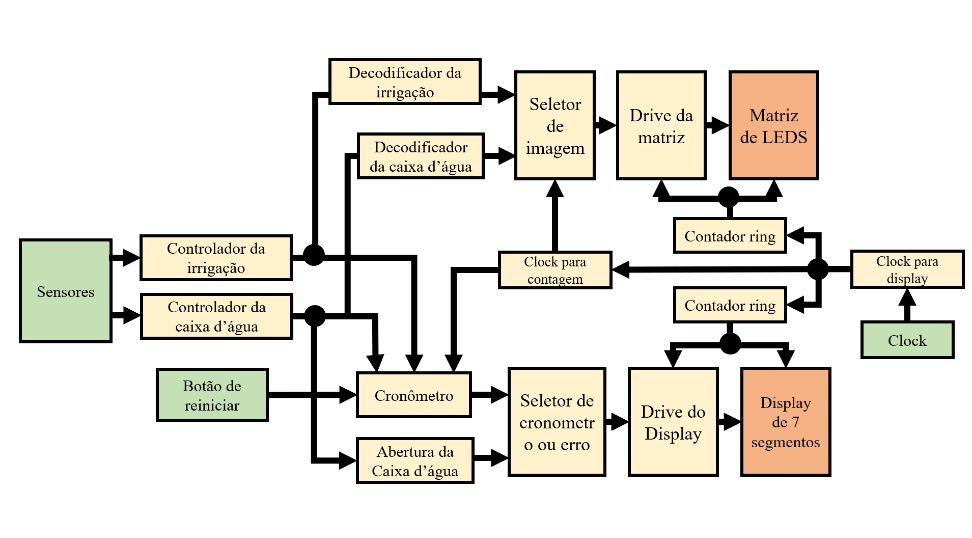
\includegraphics[width=0.75\linewidth]{fluxograma.png}
    \caption{Fluxograma geral do projeto}
    \label{fig:fluxograma}
\end{figure}

Os sensores empregados englobam tanto os sensores da caixa d'água quanto os sensores de ambiente. Os sensores da caixa d'água são categorizados em quatro níveis: crítico, baixo, médio e alto. Os sensores ambientais medem a umidade do solo, a umidade do ar e a temperatura, com a lógica inversa aplicada à temperatura. 

Os sensores da caixa d'água fornecem dados para o codificador, que converte esses dados em valores binários de dois bits, categorizando-os como crítico, baixo, médio ou alto. Além disso, esses dados são encaminhados para o sistema de erro, que verifica a regularidade entre os sensores. Caso seja detectada uma irregularidade, o sistema emite um sinal que altera a imagem do cronômetro e o estado da válvula para uma mensagem de erro exibida no \textit{display}.

A codificação gerada é transmitida ao decodificador da caixa d'água, cuja função é exibir a imagem correspondente na matriz de LEDs. Para monitorar o estado da válvula da caixa d'água, o sensor de nível alto, junto com o sistema de erro, é enviado a um módulo responsável por definir a exibição de "A" (aberto) ou "F" (fechado) no cronômetro, especificamente no \textit{display} mais à esquerda do multiplexador. 

O multiplexador, que atua como \textit{driver} do \textit{display}, seleciona qual dos quatro \textit{displays} será ativado em cada instante, com o \textit{display} mais à esquerda exibindo a informação mencionada.

No sistema de irrigação, as chaves de irrigação são processadas por um codificador que determina o modo de irrigação: aspersão ou gotejamento. Este codificador de um bit também avalia se as condições são adequadas para a irrigação, considerando o nível da caixa d'água para determinar se está em estado crítico. O codificador envia o modo de irrigação e a confirmação da irrigação ao decodificador de irrigação, que então gera a imagem correspondente na matriz de LEDs.

Para a intercalação das imagens, utiliza-se um \textit{clock} integrado à placa. Inicialmente, este \textit{clock} é enviado a um divisor de \textit{clock}, responsável por intercalar as colunas, tanto do \textit{display} quanto da matriz de LEDs, em uma frequência maior. Este \textit{clock}, então, alimenta os contadores: um \textit{ring counter }de 3 bits e um de 4 bits, sendo o de 4 bits designado para o \textit{display} e o de 3 bits para a matriz. A escolha de 3 bits para a matriz se deve ao fato de que a imagem é espelhada, exibindo duas colunas por vez, com a coluna central sendo exibida individualmente, resultando em uma exibição dual.

Posteriormente, o sinal do \textit{clock} passa por um segundo divisor de \textit{clock}, que regula a alternância entre as imagens da matriz de LEDs, dividindo o tempo igualmente entre a representação da irrigação e da caixa d'água. 

A matriz utiliza dois decodificadores, um para a caixa d'água e outro para a irrigação, que intercalam as imagens conforme o \textit{clock} mais lento. A seguir, o sinal é direcionado para o seletor, que alimenta o drive da matriz. Este drive seleciona qual coluna será exibida em cada ciclo. O contador de três bits, após passar por um decodificador que realiza a redistribuição de três entradas para cinco saídas, organiza as colunas da seguinte maneira: a saída do contador dois controla as colunas quatro e zero, a saída do contador um controla as colunas três e um, e a saída do contador zero controla a coluna central, coluna dois. Esta redistribuição é então alimentada ao drive da matriz, que ativa e desativa as colunas conforme necessário. Para o funcionamento correto, a coluna deve estar desativada enquanto a linha está ativada, permitindo uma seleção precisa. 

No sistema de decodificação, a lógica é configurar quais linhas de cada coluna serão desativadas, uma vez que o padrão é estar ativado. Assim, a operação principal é a desativação seletiva das linhas.


\subsection{Módulos}
Para a concretização do circuito conforme delineado no planejamento inicial, foram concebidos diversos módulos especializados, cada um com a finalidade de atender a objetivos técnicos específicos para o funcionamento do sistema. Esses módulos abarcam uma gama diversificada de funcionalidades. São eles: Módulos para Abastecimento de Água (\textit{Water Supply}); Módulos Utilitários (\textit{Utils}); Módulos para Matriz de LEDs (\textit{Matrix}); Módulos para Temporização (\textit{Timer}); e Módulos para Irrigação (\textit{Irrigation}).

Os módulos para a irrigação, ou tipo de rega, gerenciam os ciclos de irrigação, controlando a ativação e desativação dos mecanismos de rega conforme os requisitos de umidade do ar e do solo, além da temperatura. Estes não foram alterados na atual melhoria do projeto. Assim, não precisarão ser mencionados novamente.

No total, foram desenvolvidos 29 módulos. Para evitar a extensão excessiva do presente relatório, alguns módulos serão abordados de forma mais concisa, especialmente aqueles já discutidos no projeto anterior. Portanto, não serão repetidas as tabelas verdade e simplificações para esses módulos. O foco será nos módulos recém-criados e nos que sofreram modificações.



% -- 

\subsubsection{Water Supply, ou Válvula de abastecimento de água}

Responsáveis pelo controle e gerenciamento do nível de água. Os módulos \textit{water\_encoder} e o \textit{water\_sensors\_checker} não tiveram sua lógica alterada. A única mudança no \textit{water\_encoder} é o uso de barramento de \textit{2 bits} em sua saída de dados, o que facilita seu uso durante o código principal.

\begin{itemize}
    \item \textit{water\_supply\_controller}

O módulo \textit{water\_supply\_controller} controla a válvula de suprimento de água com base em duas condições: presença de valores conflitantes dos sensores e nível alto de água no tanque.

Quando a válvula deve ser fechada (indicada por 4'b1111):

\begin{enumerate}
    \item Há valores conflitantes provenientes dos sensores (\textit{water\_sensors\_conflicting}).

    \item O nível da água no tanque está alto (\textit{high\_water\_level}).
\end{enumerate}


A válvula é aberta (indicada por 4'b1110) somente quando não há conflitos nos sensores e o nível da água não está alto.

A lógica de controle funciona da seguinte forma:

\begin{itemize}
    \item Os três bits superiores de \textit{valvule} são sempre ativados (1) se o nível da água estiver alto.
    \item O bit menos significativo de \textit{valvule} é ativado (1) se houver valores conflitantes dos sensores ou se o nível da água estiver alto. Caso contrário, ele é desativado (0).
\end{itemize}

Isso garante que a válvula esteja fechada em condições críticas e aberta quando seguro.

\begin{equation}
\begin{split}
valvule[0] &= water\_sensors\_conflicting + high\_water\_level
\label{math:valvule}
\end{split}
\end{equation}

\begin{table}[H]
\centering
\begin{tabular}{|c|c|c|}
\hline
water\_sensors\_conflicting & high\_water\_level & valvule[0] \\ \hline
0                           & 0                  & 0          \\ \hline
0                           & 1                  & 1          \\ \hline
1                           & 0                  & 1          \\ \hline
1                           & 1                  & 1          \\ \hline
\end{tabular}
\caption{Tabela verdade dos sensores de água}
\label{tab:sensors}
\end{table}
    
\end{itemize}


\subsubsection{\textit{Utils}, ou Utilitários}
Inclui diversas funções auxiliares e de suporte que contribuem para a operação geral do sistema, ao englobar desde os redutores de \textit{clock}s, até \textit{flip-flops} e multiplexadores. Como todos são ferramentas predefinidas pela literatura, não houve a necessidade de representar as tabelas e expressões deles. Não houve alteração no \textit{multiplexer\_2x1}, o multiplexador 2x1 que foi utilizado no projeto anterior. No entanto, mais dois multiplexadores foram criados, além de 6 outros módulos. Dado que todos os módulos foram desenvolvidos com base em materiais didáticos, não se faz necessário a representação de tabelas verdade e expressões lógicas detalhadas para cada um deles. A fundamentação teórica e prática fornecida pelos materiais didáticos já garante a correta implementação dos circuitos e funcionalidades.

\begin{itemize}
    \item Multiplexadores novos

    Ambos os multiplexadores funcionam de maneira semelhante, baseados na literatura de \cite{floyd_2007_lgebra}, selecionando uma das entradas de dados com base no valor binário do contador (\textit{ring\_counter}). O valor selecionado é então transmitido para a saída \textit{out}, permitindo a escolha dinâmica de qual dado será enviado adiante no circuito. Os novos multiplexadores são os \textit{multiplexer\_3x1} e \textit{multiplexer\_4x1}, que representam respectivamente multiplexadores 3x1 e 4x1, respectivamente, adaptados para a saída do \textit{contador ring}, onde apenas um dos bits está em nível lógico alto por vez.
    
    \item  \textit{always\_on}

Foi projetado para garantir um sinal positivo constante independentemente das condições de entrada. A operação começa com a inversão da entrada a, realizada pela porta NOT, que produz a\_not. A propriedade lógica fundamental utilizada aqui é que qualquer valor lógico A somado com sua negação A' resulta em 0 (zero). Em termos da álgebra de \textit{Boole}, isso é expresso como \(A + A' = 0\).


\begin{table}[h]
    \centering
    \begin{tabular}{|c|c|>{\centering\arraybackslash}p{2mm}|c|} \hline 
         A&  A'&  & Saída\\ \hline 
         0&  0&  & x\\ \hline 
         0&  1&  & 1\\ \hline 
         1&  0&  & 1\\ \hline 
         1&  1&  & x\\ \hline
    \end{tabular}
    \caption{Tabela-verdade do módulo \textit{always_on}}
    \label{tab:always_on}
\end{table}

    
    \item \textit{clock\_divisor}

 É responsável pela redução da frequência do \textit{clock} original. Este módulo utiliza uma implementação que emprega cinco \textit{flip-flops} do tipo T conectados assincronamente, permitindo assim uma divisão do sinal de \textit{clock}. Sua saída, \textit{new\_frequency}, é definida como a saída do último \textit{flip-flop}, que agora representa a frequência reduzida do sinal de entrada. Vale ressaltar que múltiplas instâncias desse módulo fora declarada para alcançar as frequências desejadas. A equação \ref{math:clock_div} e a Figura \ref{fig:clock-div} representa a sua nova frequência de saída em relação à de entrada.

$$Nova \space Frequência = \frac{clock}{32} \label{math:clock_div}$$

\begin{figure}[H]
    \centering
    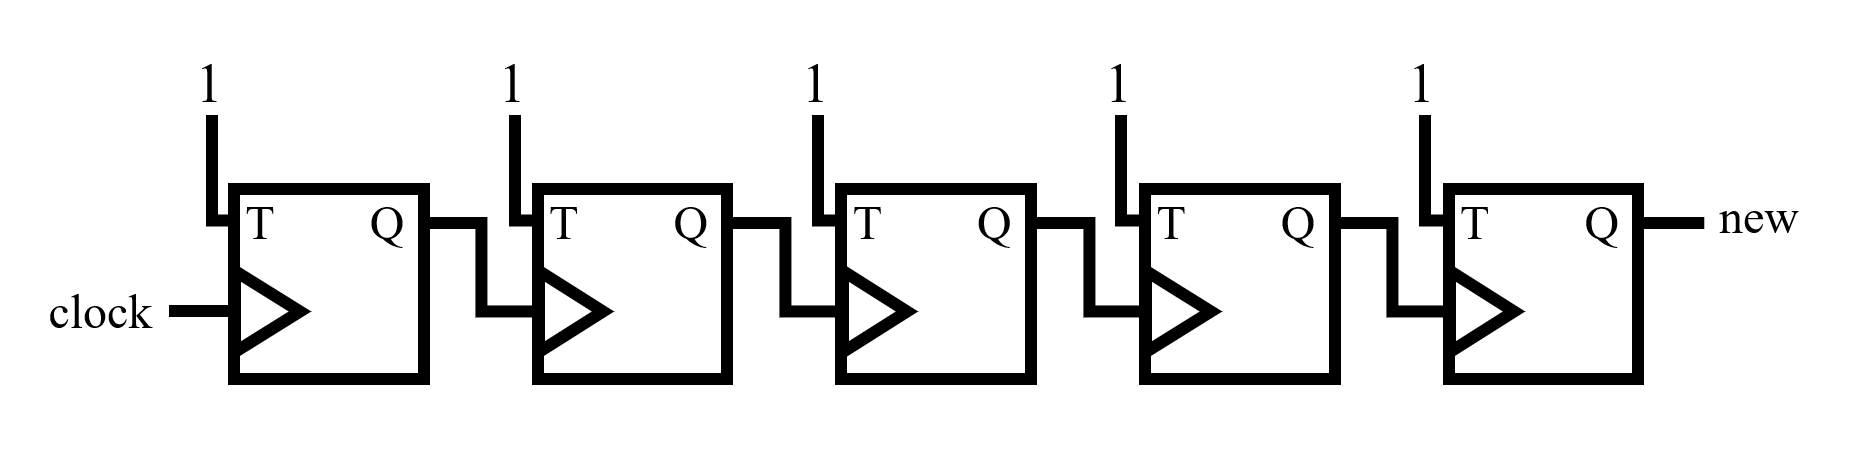
\includegraphics[width=0.5\linewidth]{clock_divisor.png}
    \caption{Esquema do divisor de clock usando Flipflops T}
    \label{fig:clock-div}
\end{figure}

    \item Flip-flops

Existem dois módulos de \textit{flipflops} no projeto, o primeiro é o \textit{flipflop\_d}, usando nos contadores, tanto os decrescentes quanto os contadores em anéis, e o segundo é o \textit{flipflop\_t}, usado para a divisão do \textit{clock}. Como o nome de ambos sugere, o primeiro é do tipo \textit{D} e o segundo do tipo \textit{T}. O primeiro contém entradas para \textit{set} e \textit{reset}, úteis para o uso de contadores, e o tipo \textit{T} contém um \textit{reset}, para caso seja necessário reiniciá-lo em alguma mudança de projeto futura.
    
    \item level\_to\_pulse

Este módulo converte um nível de sinal (0 ou 1) em um pulso curto na borda de subida do \textit{clock}. O módulo é usado duas vezes no projeto, para que um pulso seja enviado toda vez que houver comutação no modo de aspersão. Portanto, quando atualizar para Aspersão ou Gotejamento, a recontagem do temporizador é iniciada automaticamente. O \textit{level to pulse} está esquematizado na Figura \ref{fig:level-to-pulse}, e funciona da seguinte maneira:
\begin{enumerate}
    \item Armazenamento do nível: Um \textit{flip-flop} do tipo \textit{D} \textit{(flipflop\_d}) é utilizado para armazenar o nível atual do sinal de entrada \textit{level}. O \textit{clock} controla quando o \textit{flip-flop} atualiza seu valor.
    \item Negação do nível armazenado: A saída do f\textit{lip-flop} (\textit{q}) é negada através de uma porta \textit{NOT} (\textit{not\_q}). Isso significa que se \textit{q} for 1, \textit{not\_q} será 0, e vice-versa.
    \item Geração do pulso: Uma porta \textit{AND} combina o nível negado (\textit{not\_q}) com o nível original (\textit{level}). O pulso é gerado apenas quando o nível original muda de 0 para 1 (borda de subida) e o \textit{flip-flop} ainda armazena o valor antigo (0). Isso garante que o pulso seja curto e preciso.
\end{enumerate}

\begin{figure}[H]
    \centering
    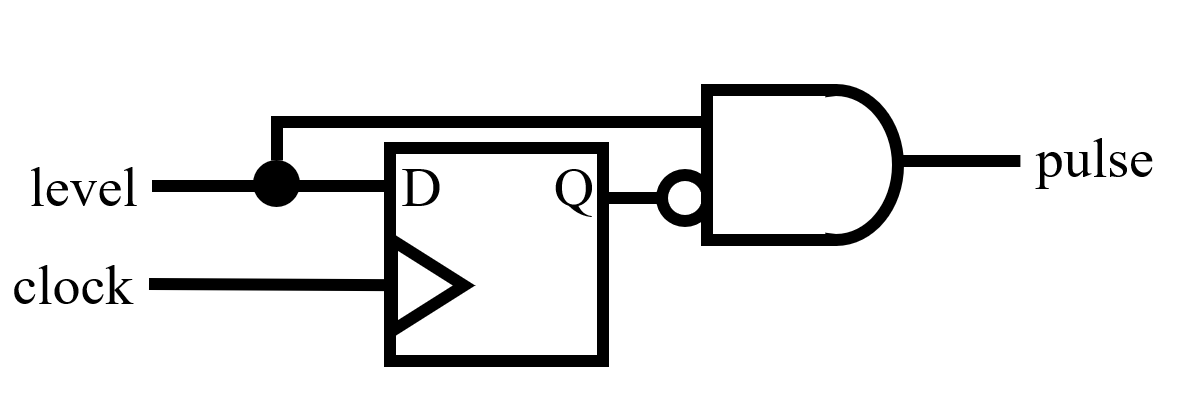
\includegraphics[width=0.5\linewidth]{level_to_pulse.png}
    \caption{Esquema do \textit{level\_to\_pulse}}
    \label{fig:level-to-pulse}
\end{figure}
    
    \item pipe

    Direciona os dados de entrada para saídas específicas do circuito. Este módulo facilita a gestão de fluxos de dados dentro do circuito digital, otimizando o processamento e a utilização dos recursos disponíveis. Como o projeto utiliza de de \textit{Verilog} estrutural ao invés de comportamental, com exceção dos \textit{flipflops}, então o pipe funciona como um \textit{assign}, onde a sinal de saída é idêntica ao sinal de entrada.

    O módulo utiliza uma porta lógica \textit{AND} para realizar essa operação. Por exemplo, em “A * A = A”, quando o sinal de entrada “A” é multiplicado por si mesmo, o resultado é igual ao próprio sinal “A”. Portanto, o sinal de saída “out” será igual ao sinal de entrada “a”. É uma operação simples, mas útil em circuitos digitais. 
\end{itemize}

\begin{table}[H]
    \centering
    \begin{tabular}{|c|c|>{\centering\arraybackslash}p{2mm}|c|} \hline 
         A&  A&  & Saída\\ \hline 
         0&  0&  & 0\\ \hline 
         0&  1&  & x\\ \hline 
         1&  0&  & x\\ \hline 
         1&  1&  & 1\\ \hline
    \end{tabular}
    \caption{Tabela-verdade do módulo \textit{pipe}}
    \label{tab:pipe}
\end{table}

\subsubsection{\textit{Matrix}, ou Matriz de LEDs}

Como no desenvolvimento do projeto anterior, a matriz de LEDs não foi utilizada, todos os módulos presentes no atual projeto que são relacionados à matriz, são novos. A ideia por de trás dos módulos da matriz é que os decodificadores enviem informações das linhas de cada coluna para o controlador, o qual chamamos de \textit{drive}, que mude a imagem mostrada conforme um contador \textit{ring de 3bits}. A escolha do contador de \textit{3 bits} para uma matriz de 5 colunas se deve ao fato da escolha das imagens mostradas serem simétricas no eixo vertical, o que reduz consideravelmente a quantidade de \textit{elementos lógicos}, já que são decodificadas apenas 3 colunas para a imagem do modo de irrigação e 2, para o nível da caixa d'água.

\begin{itemize}
    \item \textit{column\_selector}
    
É um contador de \textit{3 bits} responsável por selecionar qual coluna será exibida por vez. O contador ter \textit{3 bits} é devido ao fato de ter sido escolhido imagens espelhadas no eixo vertical para a matriz de LEDs, reduzindo assim a quantidade de recursos utilizados na sua implementação.  Assim, cada decodificador só precisa enviar informações das linhas (um barramento de 7 bits) de apenas 3 colunas. Seu circuito está representado na Figura \ref{fig:column_selector}.

\begin{figure}[H]
    \centering
    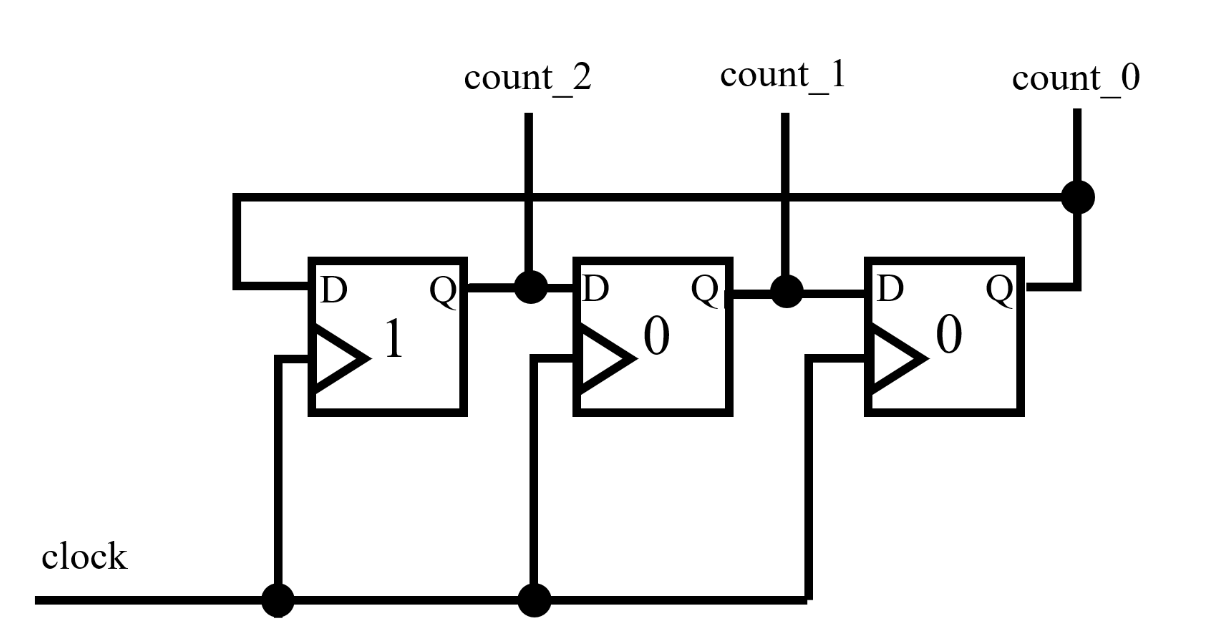
\includegraphics[width=0.5\linewidth]{column_selector.png}
    \caption{Circuito do \textit{column\_selector}}
    \label{fig:column_selector}
\end{figure}
\begin{table}[H]
    \centering
    \begin{tabular}{|c|c|>{\centering\arraybackslash}p{2mm}|c|c|c|} \hline 
         Atual&  Próximo&  & count_2& count_1&count_0\\ \hline 
         100&  010&  & 0& 1&0\\ \hline 
         010&  001&  & 0& 0&1\\ \hline 
         001&  100&  & 1& 0&0\\\hline
    \end{tabular}
    \caption{Tabela de estados do contador ring de 3 bits}
    \label{tab:3bits-ring}
\end{table}

\item \textit{matrix\_driver}

Seu funcionamento é de um multiplexador que utiliza barramentos, ao invés de sinais individuais. Assim, recebe-se 3 barramentos de 7 bits, um para cada coluna, contento informações para ativação ou não de cada linha dessa coluna, e então retorna um desses barramentos por vez, de acordo com um seletor. Sua multiplexação é feita diretamente pelo \textit{contador ring de 3 bits}, (\textit{column\_selector}) portanto apenas um dos \textit{bits} pode estar em nível lógico alto por vez. Seu circuito se encontra na Figura \ref{fig:matrix_driver}.

\begin{figure}[H]
    \centering
    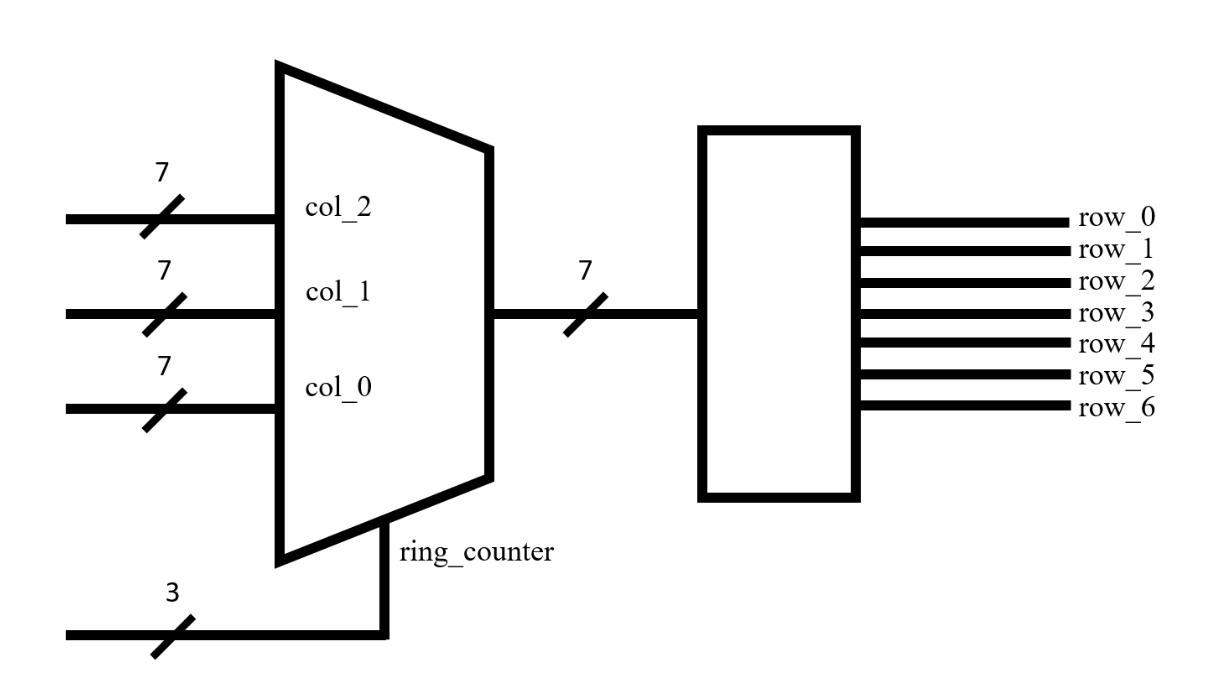
\includegraphics[width=0.5\linewidth]{matrix_driver.png}
    \caption{Circuito do \textit{matrix\_driver}}
    \label{fig:matrix_driver}
\end{figure}


    \item \textit{matrix\_ring\_decoder} 

    Desempenha a função de transformar entradas de 3 bits em saídas de 5 bits. Este decodificador possui uma característica especial, já pode ser escrito sem a presença de portas lógicas, a pesar da terem sido usadas para a implementação em \textit{Verilog} estrutural, por meio de instâncias do módulo \textit{pipe}. Sua única função é a de redistribuir cada \textit{bit} da saída do \textit{column\_selector} (\textit{3 bits}) para a as colunas da matriz de LEDs (\textit{5 bits}), espelhando-os verticalmente. Seu esquema pode ser visto na Figura \ref{fig:ring_counter}.

\begin{figure}[H]
    \centering
    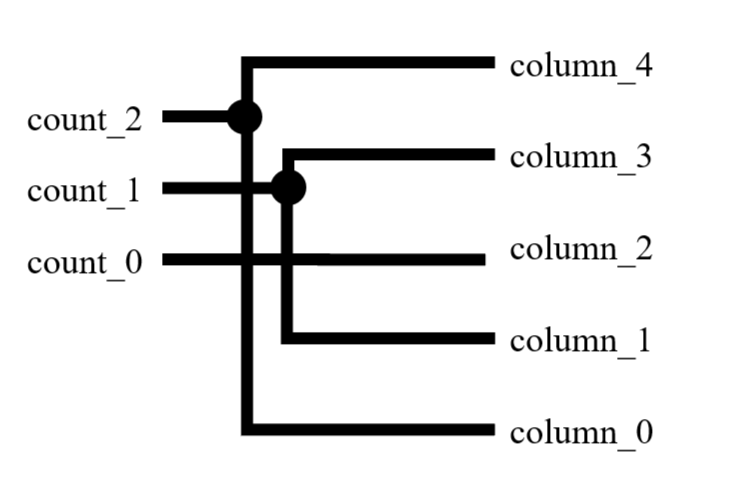
\includegraphics[width=0.5\linewidth]{image.png}
    \caption{Circuito do \textit{matrix\_ring\_decoder} }
    \label{fig:ring_counter}
\end{figure}

    \item \textit{irrigation\_mode\_decoder}

    Decodifica os sinais provenientes do sistema de irrigação, representando modos como aspersão, gotejamento, ou a ausência de irrigação na matriz de LEDs. Este módulo recebe entradas específicas dos sinais de \textit{splinker} e  \textit{irrigation}, ajustando a exibição conforme o modo de irrigação ativo.
Caso exista irrigação e o modo de aspersão esteja ativo, será decodificado a imagem de um aspersor, já caso esteja no modo de gotejamento (quando \textit{splinker} estiver em nível lógico baixo, pois são complementares), a imagem de uma gota será decodificada. Do contrário, caso não haja irrigação, será decodificado uma exclamação, independente do sinal do modo de irrigação.
A tabela verdade de cada linha e coluna pode ser vista em \ref{fig:irrigation_decoder}, enquanto a simplificação de suas expressões pode ser vista nos mapas de Karnaugh \ref{fig:irrigation-1111}, \ref{fig:irrigation-1110}, \ref{fig:irrigation-1011}, \ref{fig:irrigation-1010}. Pode ser visto em cada mapa-K a presença da numeração de sua coluna e linha no formato "coluna:linha".

\begin{equation}
\begin{split}
% valvule[0] &= water\_sensors\_conflicting + high\_water\_level
\label{math:valvule}
\end{split}
\end{equation}

\begin{figure}[H]
    \centering
    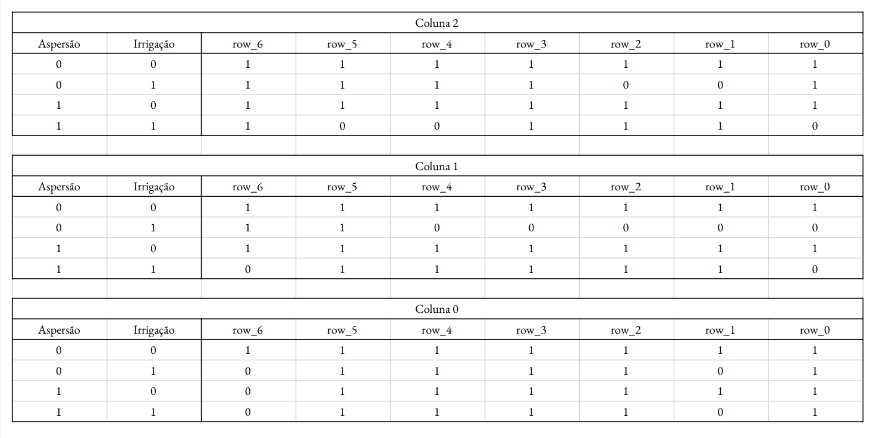
\includegraphics[width=0.9\linewidth]{irrigation_decoder.png}
    \caption{Tabelas verdade do \textit{irrigation\_decoder}}
    \label{fig:irrigation_decoder}
\end{figure}
\begin{figure}[H]
    \centering
    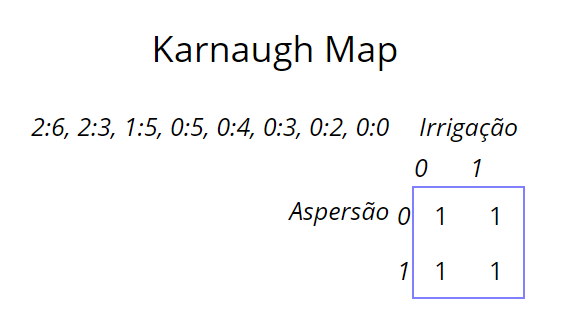
\includegraphics[width=0.5\linewidth]{irrigation-1111.png}
    \caption{Expressão: $Y = 1$}
    \label{fig:irrigation-1111}
\end{figure}
\begin{figure}[H]
    \centering
    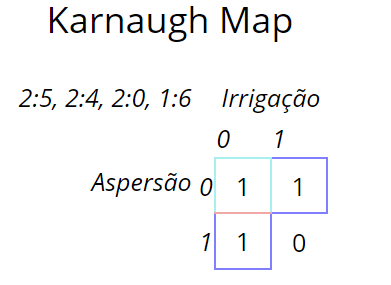
\includegraphics[width=0.4\linewidth]{kmap1110e.png}
    \caption{Expressão: $Aspersão' + Irrigação'$}
    \label{fig:irrigation-1110}
\end{figure}
\begin{figure}[H]
    \centering
    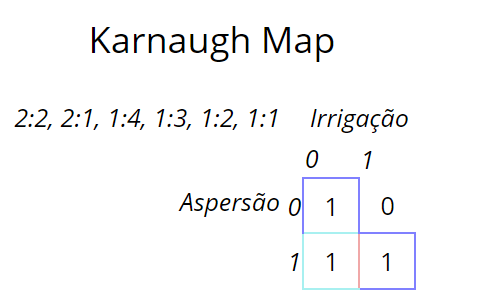
\includegraphics[width=0.45\linewidth]{irrigation-kmap1011ge.png}
    \caption{Expressão: $Irrigação' + Aspersão$}
    \label{fig:irrigation-1011}
\end{figure}
\begin{figure}[H]
    \centering
    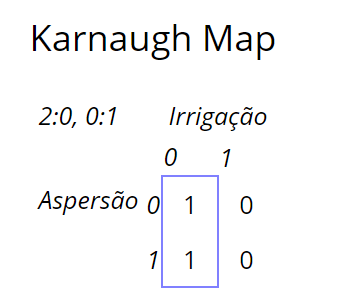
\includegraphics[width=0.35\linewidth]{irrigation-kmap-1010ge.png}
    \caption{Expressão: $Irrigação'$}
    \label{fig:irrigation-1010}
\end{figure}
    
    \item \textit{water\_level\_decoder}
    
    Recebe o nível da água codificado e verifica a presença de erros. Este módulo é projetado para retornar imagens apropriadas à matriz de LEDs, com uma característica especial que envolve o uso de um barramento de 2 bits para as colunas do meio, que são idênticas. Em caso de detecção de erro, nenhuma imagem é exibida, alertando o sistema para a necessidade de correção.
A tabela verdade contento as linhas e colunas do decodificador da matriz está disponível na Figura \ref{fig:water_level_decoder}, enquanto isso, a simplificação das expressões por meio do Mapa-K pode ser encontrado nas Figuras \ref{fig:water-1111-1111}, \ref{fig:water-1110-1111}, \ref{fig:water-1100-1111} e \ref{fig:water-1000-1111}. A posição da expressão a ser usada na matriz é representada logo acima da tabela usando o formato "coluna:linha".

\begin{figure}[H]
    \centering
    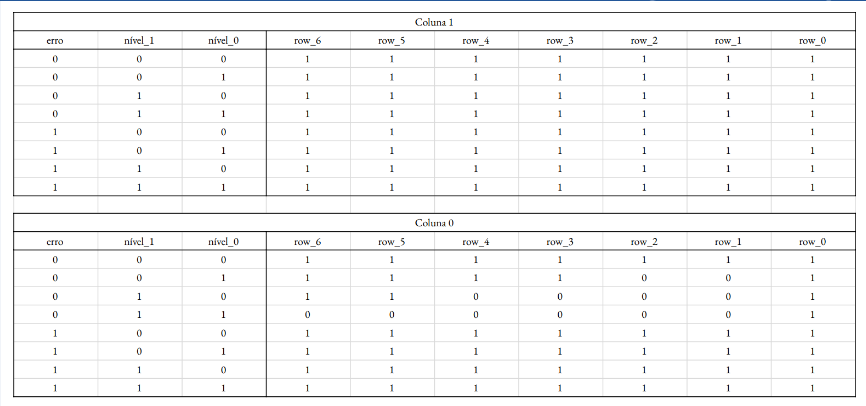
\includegraphics[width=0.9\linewidth]{water_level_decoder.png}
    \caption{Tabelas verdade do \textit{water\_level\_decoder}}
    \label{fig:water_level_decoder}
\end{figure}

\begin{figure}[H]
    \centering
    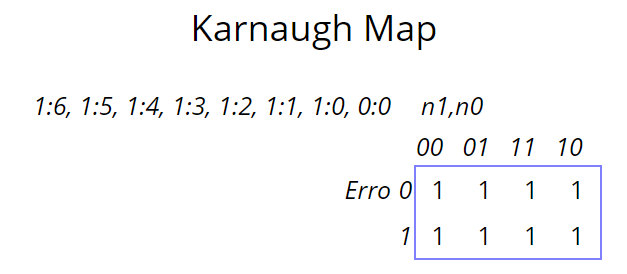
\includegraphics[width=0.5\linewidth]{water-1111-1111.png}
    \caption{Expressão: $Y = 1$}
    \label{fig:water-1111-1111}
\end{figure}
\begin{figure}[H]
        \centering
        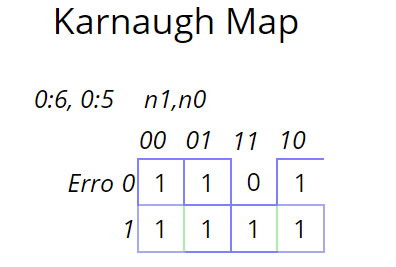
\includegraphics[width=0.35\linewidth]{water-1110-1111.png}
        \caption{Expressão: $Y = n_1' + n_0' + Erro$}
        \label{fig:water-1110-1111}
    \end{figure}    
\begin{figure}[H]
    \centering
    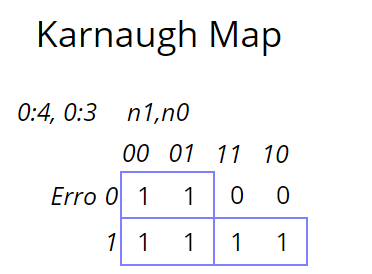
\includegraphics[width=0.3\linewidth]{water-1100-1111.png}
    \caption{Expressão: $Y = n_1' + Erro$}
    \label{fig:water-1100-1111}
\end{figure}
\begin{figure}[H]
    \centering
    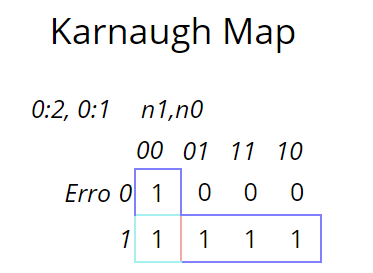
\includegraphics[width=0.3\linewidth]{water-1000-1111.png}
    \caption{Expressão: Y = $n_1'n_0' + Erro$}
    \label{fig:water-1000-1111}
\end{figure}

    \item \textit{select\_matrix\_display\_mode}

    É um multiplexador que seleciona entre as imagens representativas do modo de irrigação e as do nível da caixa d'água. Este módulo alterna entre os modos com base em um seletor controlado por um clock, permitindo uma transição fluida e sincronizada entre as diferentes informações exibidas na matriz de LEDs. Seu circuito está representado na Figura \ref{fig:select_matrix_display_mode}.

\begin{figure}[H]
    \centering
    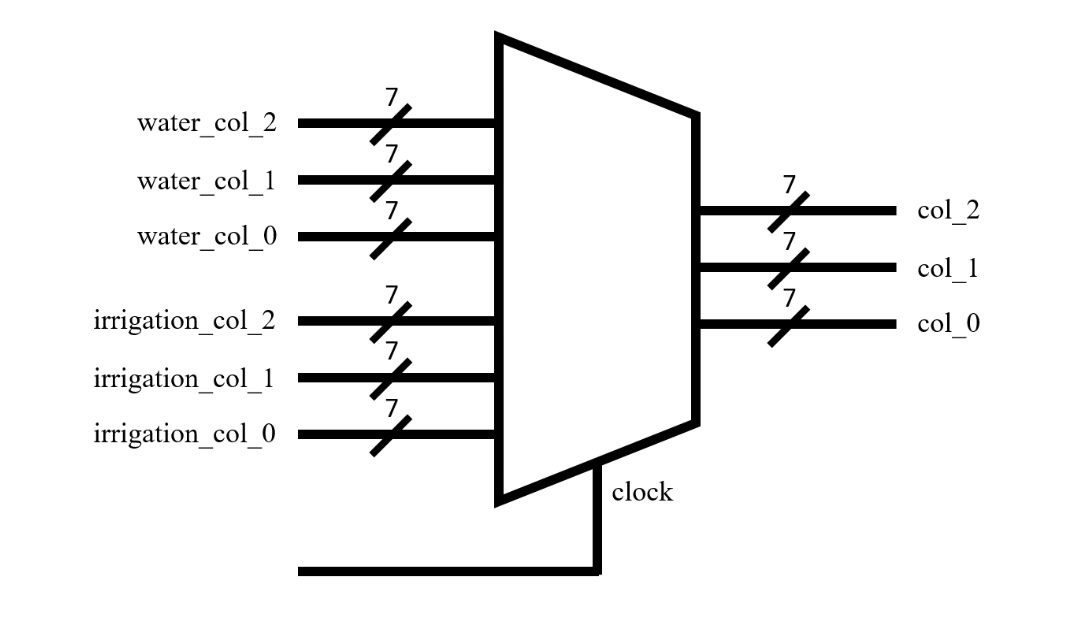
\includegraphics[width=0.5\linewidth]{select_matrix_mode.png}
    \caption{Circuito do \textit{select\_matrix\_display\_mode}}
    \label{fig:select_matrix_display_mode}
\end{figure}
    
\end{itemize}

\subsubsection{\textit{Timer}, ou Temporizador}

Implementa as funcionalidades de temporização, necessárias para visualização no display.

\begin{itemize}
    \item Contadores

A lógica de representação desses contadores utiliza 4 bits de saída para representar um BCD (Binary-Coded Decimal). Este código binário é então direcionado ao decodificador, que é responsável por interpretar e exibir os valores no display. Para a exibição no display, apenas os valores binários de 0 a 9 são utilizados, enquanto o valor 10 é descartado. Os valores binários excedentes são empregados para representar letras, proporcionando uma flexibilidade adicional na exibição de informações alfanuméricas no display.

Os flipflops dos contadores são síncronos, porém os contadores são assíncronos entre si. Dependendo dos contadores anteriores para realizar a contagem decrescente. Ao alcançar zero, o \textit{clock} que entra no contador mais à esquerda (o \textit{down\_from\_5}) é inibido, até que haja um pulso de atualização pelo módulo \textit{timer\_reseter}. O uso de três contadores que usam a quantidade mínimo necessária de \textit{flipflops} para a representação de cada dígito é importante para a redução do uso de recursos da placa. As tabelas verdade dos três contadores se encontram na Figura \ref{fig:contadores}.

    \begin{enumerate}
        \item \textit{down\_from\_9}

        O contador "down\_from\_9" é projetado para realizar contagens decrescentes de 9 a 0. Este módulo é composto por quatro flip-flops do tipo D, que juntos representam quatro bits. A saída combinada dos quatro flip-flops é utilizada para alimentar o clock do contador subsequente, o "down\_from\_3", enquanto isso, seu \textit{clock} vem da saída combinada do \textit{down\_from\_5}. Esta interconexão garante uma sincronização adequada entre os módulos de contagem.
        
        \item \textit{down\_from\_5}

        O contador "down\_from\_5" desempenha a função de contar de 5 a 0 de forma decrescente. Este módulo é constituído por três flip-flops do tipo D, representando três bits. A saída combinada dos três flip-flops é utilizada para alimentar o clock do contador "down\_from\_9", criando uma cadeia lógica de contagem decrescente.
        
        \item \textit{down\_from\_3}

        O contador "down\_from\_3" conta de 3 a 0 de forma decrescente e também é composto por dois flip-flops do tipo D, associados sincronicamente. Esse contador recebe como \textit{clock} um pulso do contador anterior (o \textit{down\_from\_9}), para quando este alcançar zero, fazendo o \textit{down\_from\_3} mudar para o próximo estado.

\end{enumerate}

\begin{figure} [H]
    \centering
    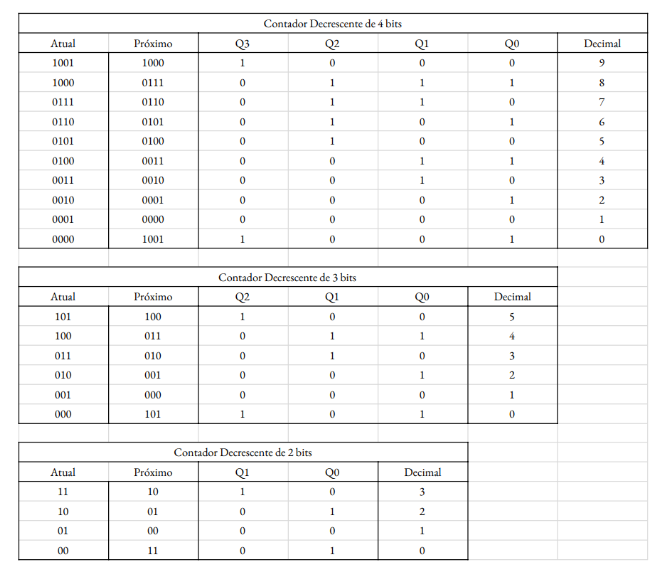
\includegraphics[width=0.75\linewidth]{contadores.png}
    \caption{Tabelas verdade dos contadores}
    \label{fig:contadores}
\end{figure}
    
        \item \textit{display\_decoder}

Este módulo converte um código binário de 4 bits em sinais de controle para um \textit{display} de sete segmentos. O decodificador também suporta a exibição das letras 'A', 'F', 'E', 'r', e 'o', além dos dígitos de 0 a 9. Vale ressaltar que a escolha do 'A' e 'F' como '1110' e '1111', respectivamente, não fora por acaso, mas uma forma de simplificar o uso, pois apenas o bit menos significativo muda entre ambos.

A entrada de 4 bits (\textit{data}) é usada para determinar quais segmentos do \textit{display} devem ser acesos para formar o caractere correspondente. Cada segmento do \textit{display} (\textit{a} até \textit{g}) é controlado por uma série de condições lógicas que dependem dos bits da entrada. Quando um bit específico da entrada está presente, os segmentos necessários são ativados para formar o caractere correspondente no \textit{display}. Sua tabela verdade se encontra na Tabela \ref{tab:display-decoder} e o mapa K de cada segmento pode ser visto nas figuras \ref{fig:seg-a} a \ref{fig:seg-g}.

\begin{table}[H]
    \centering
    \begin{tabular}{|c|c|>{\centering\arraybackslash}p{2mm}|c|c|c|c|c|c|c|c|c|c|c|} \hline  
         d_3&  d_2&  d_1& d_0& & a&b & c& d& e& f& g& &Rep.\\ \hline  
         0&  0&  0& 0 & & 0&0& 0& 0& 0& 0& 1& &0\\ \hline  
         0&  0&  0& 1& & 1&0& 0& 1& 1& 1& 1& &1\\ \hline  
         0&  0&  1& 0& & 0&0& 1& 0& 0& 1& 0& &2\\ \hline  
         0&  0&  1& 1 & & 0&0& 0& 0& 1& 1& 0& &3\\ \hline  
 0& 1& 0& 0 
& & 1& 0& 0& 1& 1& 0& 0& &4\\ \hline  
 0& 1& 0& 1
& & 0& 1& 0& 0& 1& 0& 0& &5\\ \hline  
 0& 1& 1& 0
& & 0& 1& 0& 0& 0& 0& 0& &6\\ \hline  
 0& 1& 1& 1 & & 0& 0& 0& 1& 1& 1& 1& &7\\ \hline  
 1& 0& 0& 0 
& & 0& 0& 0& 0& 0& 0& 0& &8\\ \hline  
 1& 0& 0& 1
& & 0& 0& 0& 0& 1& 0& 0& &9\\ \hline  
 1& 0& 1& 0
& & x& x& x& x& x& x& x& &\\ \hline  
 1& 0& 1& 1 & & 0& 1& 1& 0& 0& 0& 0& &E\\ \hline  
 1
& 1
& 0& 0 
& & 1& 1& 1& 1& 0& 1& 0& &r\\ \hline  
 1
& 1
& 0& 1
& & 1& 1& 0& 0& 0& 1& 0& &o\\ \hline  
 1
& 1
& 1& 0
& & 0& 0& 0& 1& 0& 0& 0& &A\\ \hline  
 1& 1& 1& 1 & & 0& 1& 1& 1& 0& 0& 0& &F\\ \hline 
    \end{tabular}
    \caption{Tabela da decodificação do \textit{display} de 7 segmentos}
    \label{tab:display-decoder}
\end{table}

\begin{figure} [H]
    \centering
    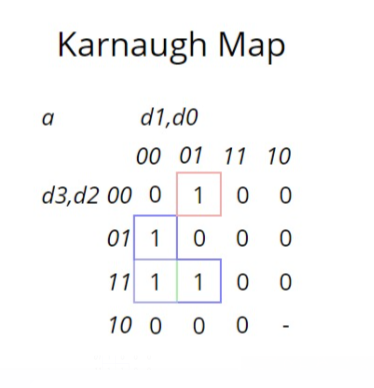
\includegraphics[width=0.3\linewidth]{a.png}
    \caption{Segmento \textit{a}}
    \label{fig:seg-a}
\end{figure}
$$
a = d_3'd_2'd_1'd_0 + d_2d_1'd_0' + d_3d_2d_1' 
$$

\begin{figure} [H]
    \centering
    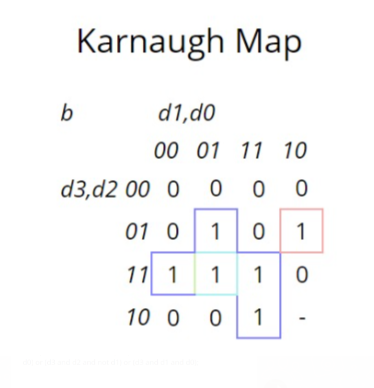
\includegraphics[width=0.3\linewidth]{b.png}
    \caption{Segmento \textit{b}}
    \label{fig:seg-b}
\end{figure}
$$
b = d_2d_1'd_0 + d_3'd_2d_1d_0' + d_3d_2d_1' + d_3d_1d_0
$$
\begin{figure} [H]
    \centering
    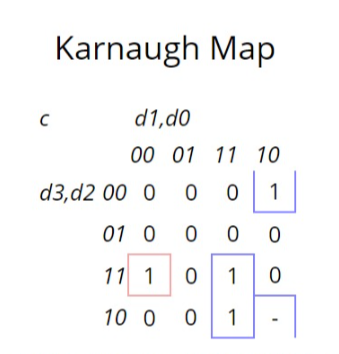
\includegraphics[width=0.3\linewidth]{c.png}
    \caption{Segmento \textit{c}}
    \label{fig:seg-c}
\end{figure}
$$
c = d_2'd_1d_0' + d_3d_2d_1'd_0' + d_3d_1d_0
$$

\begin{figure} [H]
    \centering
    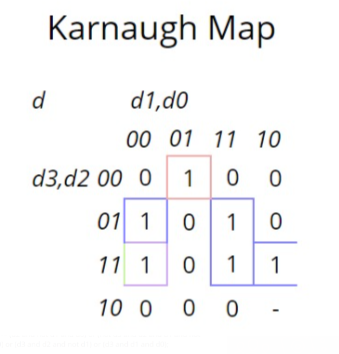
\includegraphics[width=0.3\linewidth]{d.png}
    \caption{Segmento \textit{d}}
    \label{fig:seg-d}
\end{figure}
$$
d = d_3'd_2'd_1'd_0 + d_2d_1'd_0' + d_2d_1d_0 + d_3d_2d_0' 
$$
\begin{figure} [H]
    \centering
    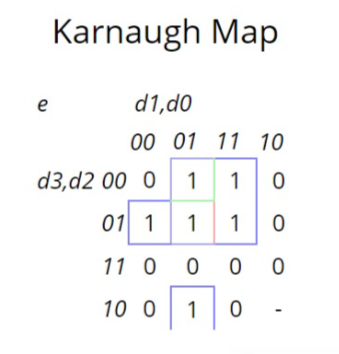
\includegraphics[width=0.3\linewidth]{e.png}
    \caption{Segmento \textit{e}}
    \label{fig:seg-e}
\end{figure}
$$
e = d_3'd_0 + d_3'd_2d_1' + d_2'd_1'd_0 
$$
\begin{figure} [H]
    \centering
    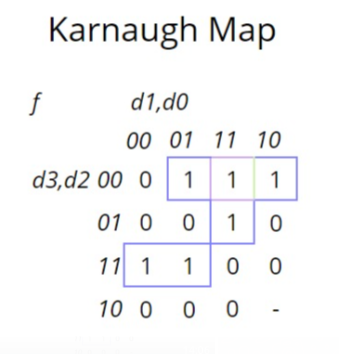
\includegraphics[width=0.3\linewidth]{f.png}
    \caption{Segmento \textit{f}}
    \label{fig:seg-f}
\end{figure}
$$
f = d_3'd_2'd_0 + d_3'd_1d_0 + d_3d_2d_1' + d_3'd_2'd_1
$$

\begin{figure}[H]
    \centering
    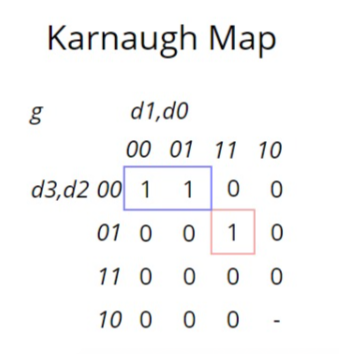
\includegraphics[width=0.3\linewidth]{g.png}
    \caption{Segmento \textit{g}}
    \label{fig:seg-g}
\end{figure}

$$
g = d_3'd_2'd_1' + d_3'd_2d_1d_0
$$

    \item \textit{display\_selector}

O seletor de \textit{display} funciona de forma muito similar ao \textit{column\_selector} descrito anteriormente para a matriz de LEDs, sendo esse um contador do tipo \textit{ring de 4bits}. Sua função é a de selecionar qual dos dígitos será mostrado por vez no \textit{display} de sete segmentos, o que permite que sejam mostradas todas as informações. Para isso, recebe-se um \textit{clock} que seja alto suficiente para que pareça uma imagem estática aos olhos humanos, quando na verdade apenas um dos dígitos é exibido por vez. Seu esquema se encontra na Figura \ref{fig:display-selector} e sua tabela de estados na Tabela \ref{tab:4bits-ring}.

\begin{figure}[H]
    \centering
    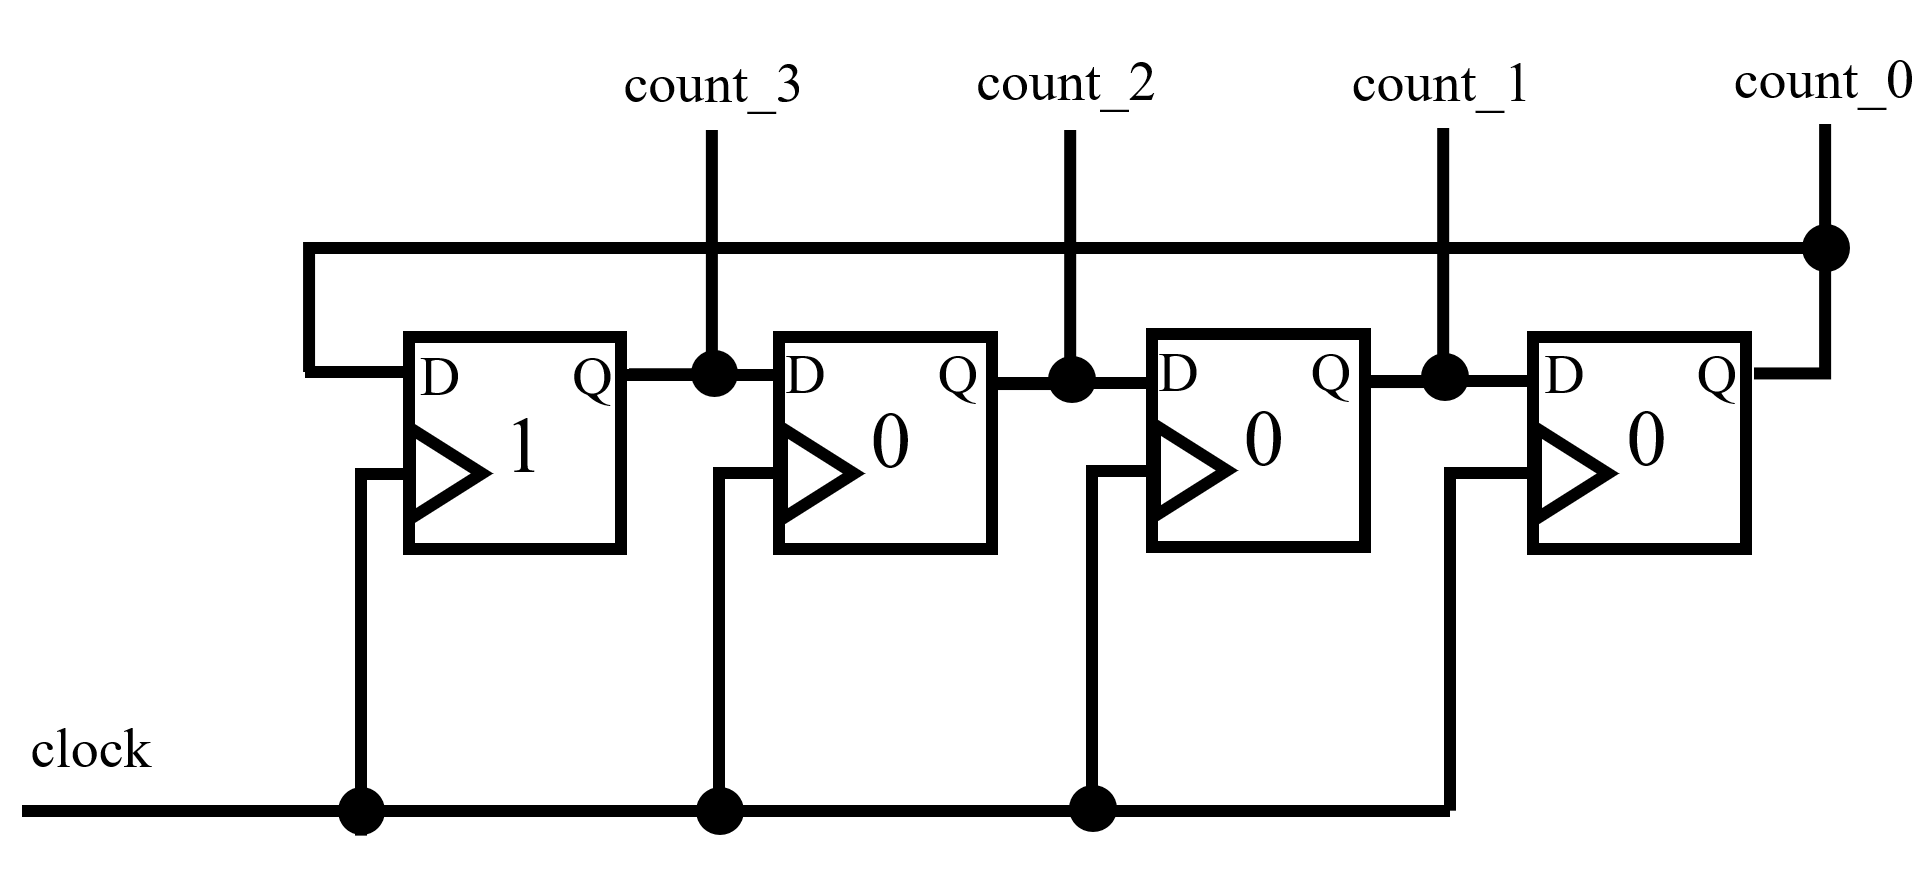
\includegraphics[width=0.5\linewidth]{display_selector.png}
    \caption{Esquema do \textit{display\_selector}}
    \label{fig:display-selector}
\end{figure}

\begin{table}[H]
    \centering
    \begin{tabular}{|c|c|>{\centering\arraybackslash}p{2mm}|c|c|c|c|} \hline 
         Atual&  Próximo&  & count_3& count_2& count_1&count_0\\ \hline 
         1000&  0100&  & 0 & 1& 0&0\\ \hline 
         0100&  0010&  & 0& 0& 1&0\\ \hline 
         0010&  0001&  & 0& 0& 0&1\\ \hline 
         0001&  1000&  & 1 & 0& 0&0\\ \hline
    \end{tabular}
    \caption{Tabela de estados do contador ring de 4 bits}
    \label{tab:4bits-ring}
\end{table}

    \item \textit{display\_driver}

    seleciona um conjunto de dados de entrada entre quatro possíveis ($data_3$, $data_2$, $data_1$, $data_0$) com base no valor do \textit{ring\_counter} e envia o conjunto selecionado para a saída out. Utiliza quatro multiplexadores 4x1 para fazer essa seleção, um para cada bit dos dados de entrada, permitindo que diferentes dados sejam exibidos em diferentes momentos conforme o valor do contador de anel. O driver recebe informações de instâncias do \textit{error\_or\_info}, responsável por intercalar entre uma mensagem de erro ou o representação padrão do cronômetro juntamente da abertura da caixa d'água.

Assim, $data_3$ pode receber a informação correspondente aos caracteres 'A' ou 'E', $data_2$ o dígito da dezena de minutos do contador ou o caractere 'r', $data_1$ o dígito da unidade de minutos ou 'r', enquanto $data_0$, a dezena de segundos ou o caractere 'o'. Seu esquema se encontra na Figura \ref{fig:display-driver}.

\begin{figure}[H]
    \centering
    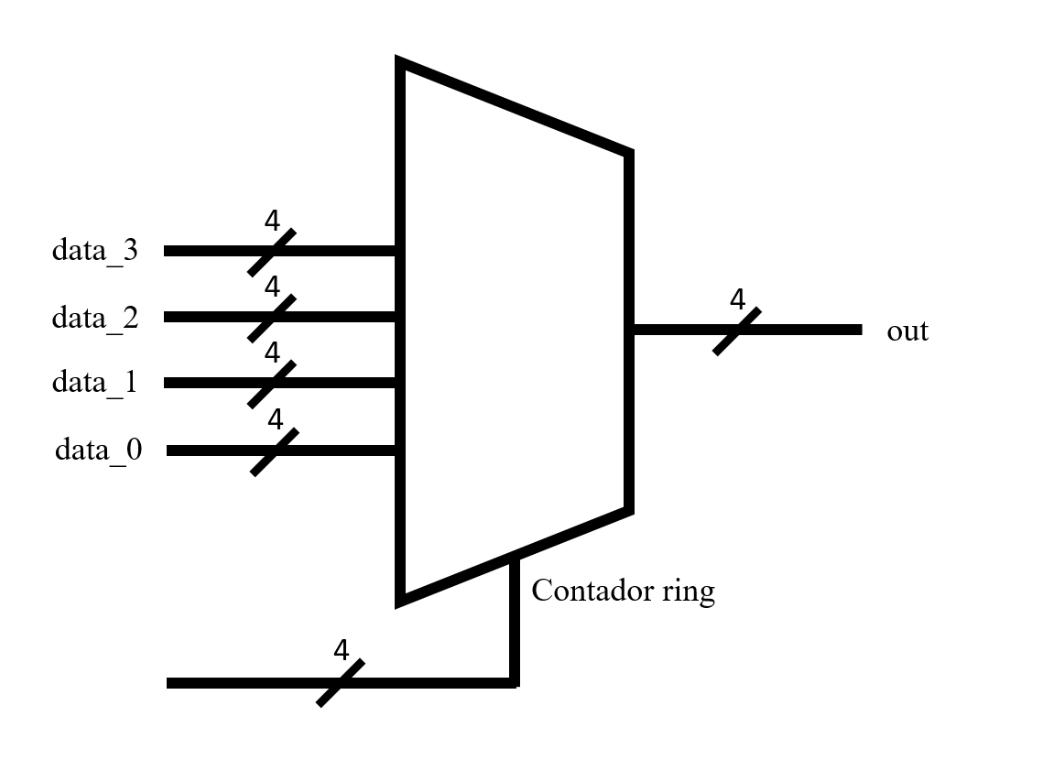
\includegraphics[width=0.5\linewidth]{display_driver.png}
    \caption{Esquema do \textit{display\_driver}}
    \label{fig:display-driver}
\end{figure}

    \item \textit{error\_or\_info}

    O módulo \textit{error\_or\_info} seleciona entre dois conjuntos de dados de entrada (\textit{info} e \textit{error}) com base no sinal \textit{has\_error}. Se \textit{has\_error} for verdadeiro, a saída out exibirá os dados de error; caso contrário, exibirá os dados de \textit{info}. Sua visualização se enccontra na Figura \ref{fig:error-or-info}. Ele usa multiplexadores 2x1 para fazer essa seleção para cada bit dos dados de entrada, permitindo a exibição de mensagens de erro ou informação conforme a necessidade. Quatro instâncias desse módulo são usadas no projeto, uma para cada dígito do mostrador de 7 segmentos.

\begin{figure}[H]
    \centering
    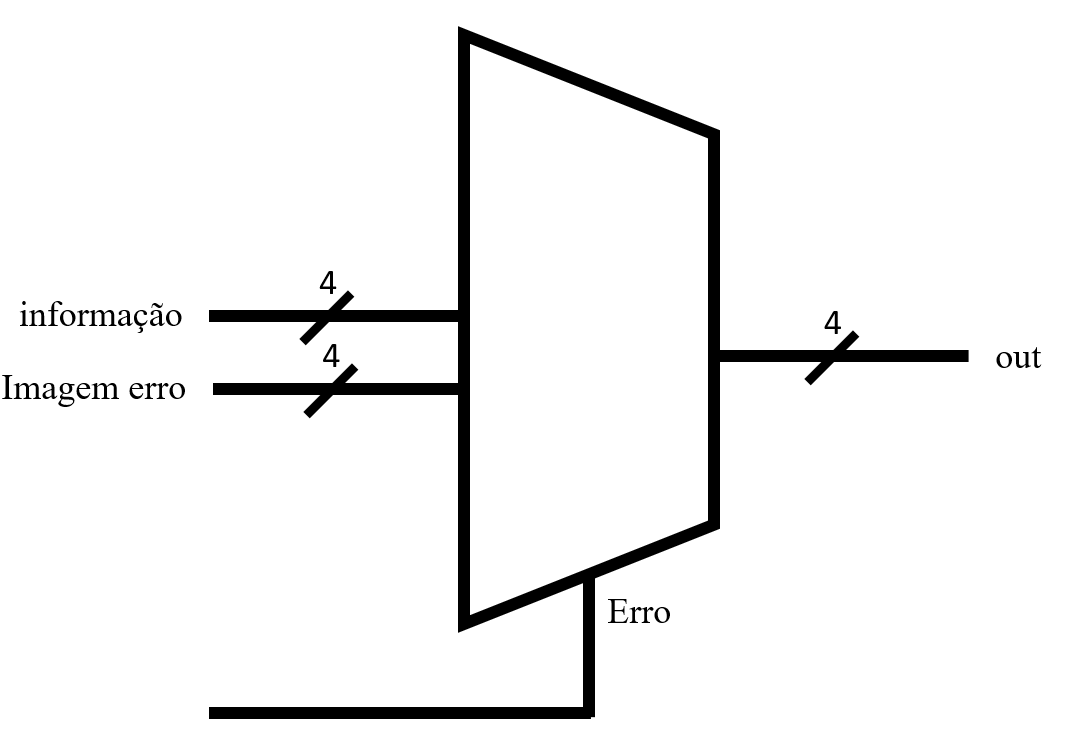
\includegraphics[width=0.5\linewidth]{error_or_info.png}
    \caption{Esquema do \textit{error\_or\_info}}
    \label{fig:error-or-info}
\end{figure}

    \item \textit{set\_display\_init}

    O módulo \textit{set\_display\_init} configura os valores iniciais dos \textit{displays} de minutos e segundos dependendo do modo de operação (\textit{splinker\_mode\_on}) e do sinal de reinício (\textit{recount}).

    \begin{enumerate}
        \item Quando \textit{splinker\_mode\_on} é verdadeiro, ele configura os \textit{displays} de minutos e segundos para os valores correspondentes ao modo "Splinker" ("0011 0000 0000", "3 0 0" em decimal).
        \item Quando \textit{splinker\_mode\_on} é falso (modo "Dripper"), ele configura os \textit{displays} para os valores do modo "Dripper" ("0001 0101 0000", "1 5 0" em decimal).
        \item \textit{recount} é utilizado para indicar quando os \textit{flipflops} devem ser configurados para o valor inicial novamente.
    \end{enumerate}

    O circuito utiliza portas lógicas para determinar os valores específicos que devem ser enviados aos \textit{displays} dos minutos (\textit{minutes\_d\_setter}, \textit{minutes\_u\_setter}, \textit{minutes\_d\_resetter}, \textit{minutes\_u\_resetter}) e segundos (\textit{seconds\_d\_resetter}) dependendo do modo de operação e do sinal de reinício. As Tabelas \ref{tab:Dezena de minutos} a \ref{tab:sets e resets} mostram as tabelas verdade dos Setters e Resetters de cada dígito do temporizador.


\begin{table}[H]
\centering
\begin{tabular}{| c  |c  |c  |c |c |c  |c  |c |c |c |}
\hline
\multicolumn{10}{|c|}{Dezena de minutos} \\
\hline
Recontar& Aspersão& \multicolumn{4}{|c|}{Setter} & \multicolumn{4}{|c|}{Resetter} \\
\hline
 &  & set_3& set_2& set_1& set_0& reset_3& reset_2& reset_1& reset_0\\ \hline 
0 & 0 & 0 & 0 & 0 & 0 & 0 & 0 & 0 & 0 \\ \hline 
0 & 1 & 0 & 0 & 0 & 0 & 0 & 0 & 0 & 0 \\ \hline 
1 & 0 & 0 & 0 & 1 & 1 & 1 & 1 & 0 & 0 \\ \hline
1 & 1 & 0 & 0 & 0 & 1 & 1 & 1 & 1 & 0 \\ \hline

\end{tabular}
\caption{Tabela verdade para a dezena de minutos}
\label{tab:Dezena de minutos}
\end{table}

\begin{table}[H]
    \centering
    \begin{tabular}{|c|>{\centering\arraybackslash}p{0.07\linewidth}|>{\centering\arraybackslash}p{0.07\linewidth}|>{\centering\arraybackslash}p{0.07\linewidth}|>{\centering\arraybackslash}p{0.07\linewidth}|>{\centering\arraybackslash}p{0.07\linewidth}|>{\centering\arraybackslash}p{0.07\linewidth}|>{\centering\arraybackslash}p{0.07\linewidth}|>{\centering\arraybackslash}p{0.07\linewidth}|} \hline 
          Saída&set_3&  set_2&  set_1&  set_0&  reset_3&  reset_2&  reset_1& reset_0\\ \hline 
          Expressão&0&  0&  RA'&  RA' + RA
 = 
R&  RA' + RA
=
R&  RA' + RA
=
R&  RA& 0\\ \hline
    \end{tabular}
    \caption{\textit{Set}s e \textit{reset}s das unidades de minutos}
    \label{tab:my_label}
\end{table}
 
\begin{table}[H]
\centering


\begin{tabular}{| c  |c  |c  |c |c |c  |c  |c |c |c |}
\hline
\multicolumn{10}{|c|}{Unidade de minutos} \\
\hline
Recontar& Aspersão& \multicolumn{4}{|c|}{Setter} & \multicolumn{4}{|c|}{Resetter} \\
\hline
 &  & set_3& set_2& set_1& set_0& reset_3& reset_2& reset_1& reset_0\\ \hline 
0 & 0 & 0 & 0 & 0 & 0 & 0 & 0 & 0 & 0 \\ \hline 
0 & 1 & 0 & 0 & 0 & 0 & 0 & 0 & 0 & 0 \\ \hline 
1 & 0 & 0 & 0 & 0 & 0 & 1 & 1 & 1 & 1 \\ \hline
1 & 1 & 0 & 1 & 0 & 1 & 1 & 0 & 1 & 0 \\ \hline

\end{tabular}
\caption{Tabela verdade para a unidade de minutos}
\label{tab:my_table}
\end{table}
\begin{table}[H]
    \centering
    \begin{tabular}{|c|>{\centering\arraybackslash}p{0.07\linewidth}|>{\centering\arraybackslash}p{0.07\linewidth}|>{\centering\arraybackslash}p{0.07\linewidth}|>{\centering\arraybackslash}p{0.07\linewidth}|>{\centering\arraybackslash}p{0.07\linewidth}|>{\centering\arraybackslash}p{0.07\linewidth}|>{\centering\arraybackslash}p{0.07\linewidth}|>{\centering\arraybackslash}p{0.07\linewidth}|} \hline 
          Saída&set_3&  set_2&  set_1&  set_0&  reset_3&  reset_2&  reset_1& reset_0\\ \hline 
          Expressão&0&  RA&  0&  RA&  RA' + RA
=
R&  RA'&  RA' + RA
=
R& RA'\\ \hline
    \end{tabular}
    \caption{\textit{Set}s e \textit{reset}s das unidades de minutos}
    \label{tab:my_label}
\end{table}
\begin{table}[H]
\centering

\begin{tabular}{| c  |c  |c  |c |c |c  |c  |c |c |c |}
\hline
\multicolumn{10}{|c|}{Dezena de segundos} \\
\hline
Recontar& Aspersão& \multicolumn{4}{|c|}{Setter} & \multicolumn{4}{|c|}{Resetter} \\
\hline
 &  & set_3& set_2& set_1& set_0& reset_3& reset_2& reset_1& reset_0\\ \hline 
0 & 0 & 0 & 0 & 0 & 0 & 0 & 0 & 0 & 0 \\ \hline 
0 & 1 & 0 & 0 & 0 & 0 & 0 & 0 & 0 & 0 \\ \hline 
1 & 0 & 0 & 0 & 0 & 0 & 1 & 1 & 1 & 1 \\ \hline
1 & 1 & 0 & 0 & 0 & 0 & 1 & 1 & 1 & 1 \\ \hline

\end{tabular}
\caption{Tabela verdade da dezena dos segundos}
\label{tab:my_table}
\end{table}
\begin{table}[H]
    \centering
    \begin{tabular}{|c|>{\centering\arraybackslash}p{0.07\linewidth}|>{\centering\arraybackslash}p{0.07\linewidth}|>{\centering\arraybackslash}p{0.07\linewidth}|>{\centering\arraybackslash}p{0.07\linewidth}|>{\centering\arraybackslash}p{0.07\linewidth}|>{\centering\arraybackslash}p{0.07\linewidth}|>{\centering\arraybackslash}p{0.07\linewidth}|>{\centering\arraybackslash}p{0.07\linewidth}|} \hline 
          Saída&set_3&  set_2&  set_1&  set_0&  reset_3&  reset_2&  reset_1& reset_0\\ \hline 
          Expressão&0&  0&  0&  0&  RA' + RA = R&  RA' + RA = R&  RA' + RA = R& RA' + RA = R\\ \hline
    \end{tabular}
    \caption{\textit{Set}s e \textit{reset}s dos segundos}
    \label{tab:sets e resets}
\end{table}

    \item \textit{timer\_reseter}
    
    O módulo \textit{timer\_reseter} gera um sinal de \textit{reset} para o temporizador com base em várias condições de entrada relacionadas ao sistema de irrigação. Ele é responsável por indicar que o temporizador deve refazer uma contagem, voltando ao estado inicial. Para isso, seu sinal deve ser enviado pata o \textit{set\_display\_init}, permitindo a atualização dos \textit{flipflops} dos contadores.

    O sinal \textit{reset} é ativado se ocorrer uma das seguintes situações:

        \begin{enumerate}
            \item O sistema de irrigação está desligado (\textit{irrigation\_off}).
            \item Um botão de \textit{reset} foi pressionado e liberado (\textit{button\_released}).
            \item Há valores conflitantes (\textit{conflicting\_values}).
            \item Um pulso de comutação do sistema de irrigação é detectado (\textit{irrigation\_switch\_pulse}).

        \end{enumerate}

Esse módulo é importante para que se possa retomar a contagem do temporizador, atualizando-o sempre que uma dessas condições acima sejam atendidas. Vale ressaltar que em alguns casos, ele é capaz de travar o temporizador no estado inicial, que pode ser de 30 minutos ou 15 minutos, como é o caso de valores conflitantes e irrigação inexistente. Seu esquema pode ser visualizado na Figura \ref{fig:timer_reseter}.

\end{itemize}

\begin{figure} [H]
    \centering
    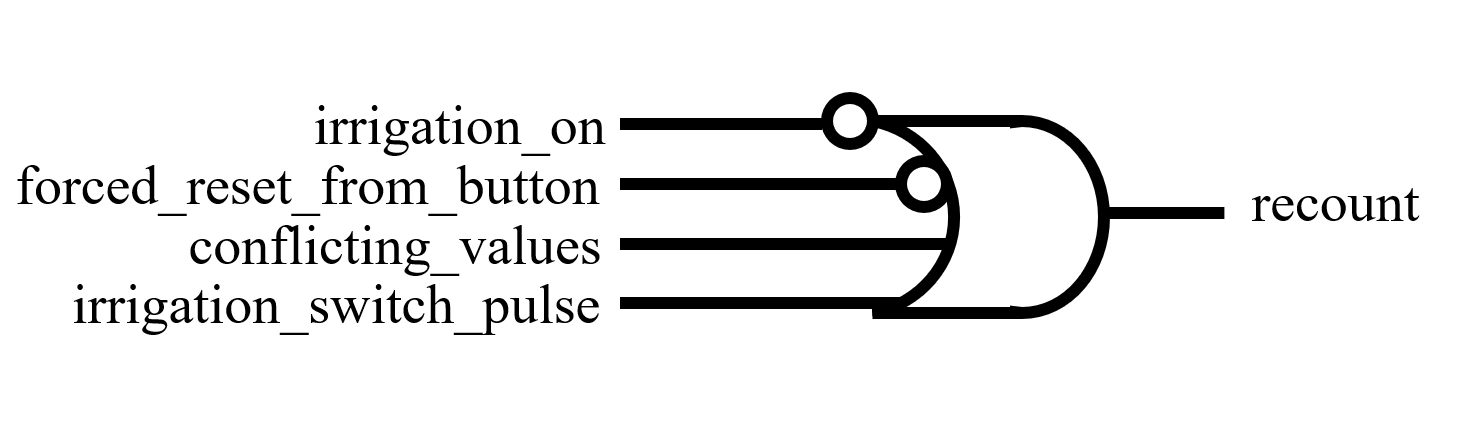
\includegraphics[width=0.5\linewidth]{reseter.png}
    \caption{Esquema do \textit{timer\_reseter}}
    \label{fig:timer_reseter}
\end{figure}

% --


\subsection{Pinagem}

Para o presente circuito, preservaram-se diversas entradas do projeto precedente, incluindo as chaves pinadas associadas aos níveis da caixa d'água, bem como os sensores de umidade e temperatura. Contudo, houve a introdução de novas entradas, destacando-se os sinais de \textit{reset}, designados como Pulso 3 e Pulso 2, além do sinal de \textit{clock}.

Toda a pinagem, com as devidas atualizações podem ser observadas na Tabela \ref{tab:componentes-pinos}.

\begin{table}[H]
\centering
\begin{tabular}{|c|c|c|}
\hline
\textbf{Componente} & \textbf{Nome} & \textbf{Pino} \\ \hline
\multicolumn{3}{|c|}{\textbf{Entradas}} \\ \hline
Switch & Temperatura & CH5 (30) \\ \hline
Switch & Umidade do Ar & CH4 (34) \\ \hline
Switch & Umidade da Terra & CH3 (36) \\ \hline
Switch & Nível Alto da Água & CH2 (38) \\ \hline
Switch & Nível Médio da Água & CH1 (40) \\ \hline
Switch & Nível Baixo da Água & CH0 (42) \\ \hline
Botão & Pulso 3 & B0 (52) \\ \hline
Botão & Pulso 2 & B1 (50) \\ \hline
Clock & Clock & 12 \\ \hline
\multicolumn{3}{|c|}{\textbf{Saídas}} \\ \hline
LED & Indicador Válvula Abastecimento & LED0 (54) \\ \hline
LED & Contador 2 & LED2 (57) \\ \hline
LED & Contador 1 & LED3 (61) \\ \hline
LED & Contador 0 & LED4 (67) \\ \hline
LED & Válvula Gotejadora & LED8 (75) \\ \hline
LED & Bomba Aspersora & LED9 (76) \\ \hline
LED & Alarme (Vermelho) & Red Led (86) \\ \hline
\multicolumn{3}{|c|}{\textbf{Display 7 Segmentos}} \\ \hline
Cátodo & Segmento A & 7 SEG-A (90) \\ \hline
Cátodo & Segmento B & 7 SEG-B (70) \\ \hline
Cátodo & Segmento C & 7 SEG-C (41) \\ \hline
Cátodo & Segmento D & 7 SEG-D (98) \\ \hline
Cátodo & Segmento E & 7 SEG-E (100) \\ \hline
Cátodo & Segmento F & 7 SEG-F (92) \\ \hline
Cátodo & Segmento G & 7 SEG-G (39) \\ \hline
Ânodo Comum & Display 0 (Dígito mais à direita) & 7 SEG-D1 (37) \\ \hline
Ânodo Comum & Display 1 & 7 SEG-D2 (68) \\ \hline
Ânodo Comum & Display 2 & 7 SEG-D3 (66) \\ \hline
Ânodo Comum & Display 3 (Dígito mais à esquerda) & 7 SEG-D4 (88) \\ \hline
Ponto Decimal & & 7 SEG-P (96) \\ \hline
\multicolumn{3}{|c|}{\textbf{Matriz}} \\ \hline
Coluna & Coluna 0 & 97 \\ \hline
Coluna & Coluna 1 & 99 \\ \hline
Coluna & Coluna 2 & 95 \\ \hline
Coluna & Coluna 3 & 82 \\ \hline
Coluna & Coluna 4 & 78 \\ \hline
Linha & Linha 0 & 85 \\ \hline
Linha & Linha 1 & 83 \\ \hline
Linha & Linha 2 & 84 \\ \hline
Linha & Linha 3 & 87 \\ \hline
Linha & Linha 4 & 81 \\ \hline
Linha & Linha 5 & 91 \\ \hline
Linha & Linha 6 & 89 \\ \hline
\end{tabular}
\caption{Tabela de componentes e pinos}
\label{tab:componentes-pinos}
\end{table}


% --

\subsection{Ferramentas Auxiliares}

Para simplificar o processo de desenvolvimento do projeto, foram empregados dois arquivos Python: o \textit{clean.py} e o \textit{update\_config.py}. Ambos desempenharam papéis importantes no projeto anterior e foram novamente utilizados nesta iteração.


\section{Resultados}
% temp
No desenvolvimento do projeto, visando a utilização otimizada dos recursos da CPLD, foram adotadas diversas estratégias, como o espelhamento de colunas na matriz de LEDs, o que resultou em uma significativa redução no consumo de Elementos Lógicos (LEs).

No total, foram utilizados 104 dos 240 Elementos Lógicos disponíveis e 41 dos 80 pinos da CPLD. A utilização detalhada dos elementos lógicos é apresentada nas Figuras \ref{fig:LEs} e \ref{fig:LUTs}.

\begin{figure}[H]
    \centering
    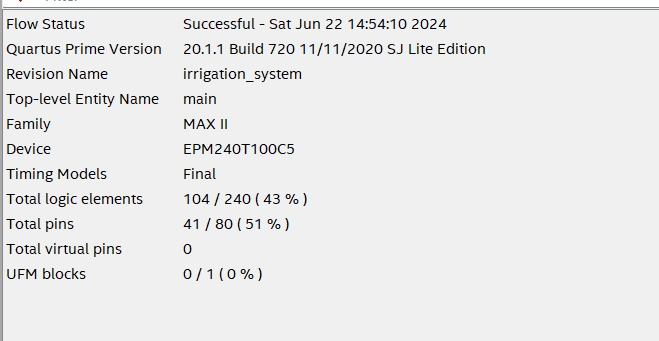
\includegraphics[width=0.65\linewidth]{LEs.png}
    \caption{Utilização dos Elementos Lógicos}
    \label{fig:LEs}
\end{figure}

\begin{figure} [H]
    \centering
    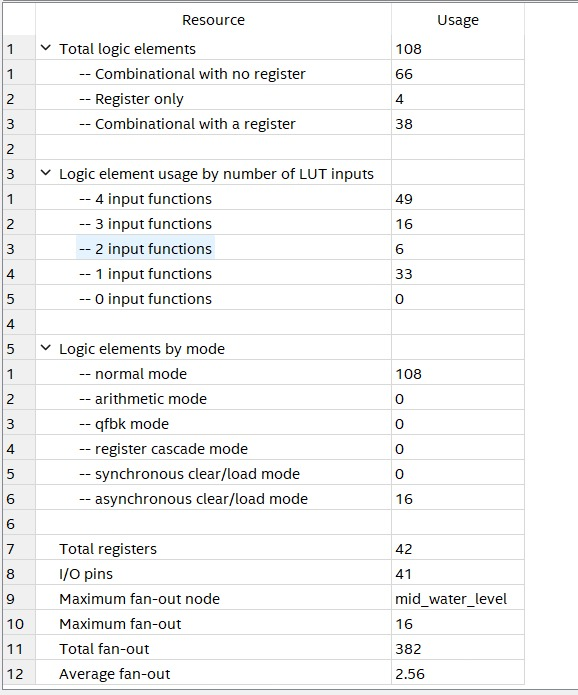
\includegraphics[width=0.6\linewidth]{LUTs.png}
    \caption{Uso dos recursos da CPLD}
    \label{fig:LUTs}
\end{figure}

\subsection{Imagens da Placa}

Conforme mencionado na Seção 1.5 (Pinagem), foram adotadas diversas formas de representar as entradas para ilustrar de maneira clara cada situação possível do ambiente.

Primeiramente, a matriz de LEDs é utilizada para representar tanto o nível da caixa d'água (Figuras \ref{fig:critico}, \ref{fig:baixo}, \ref{fig:meio} e \ref{fig:alto}), quanto o tipo de irrigação (Figuras \ref{fig:asp} e \ref{fig:got}). Essas duas informações são alternadas periodicamente na mesma matriz, permitindo que sejam visualizadas integralmente.

\begin{figure}[H]
    \centering
    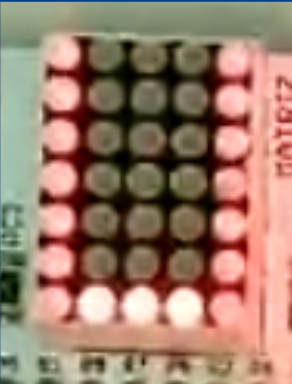
\includegraphics[width=0.3\linewidth]{critico.png}
    \caption{Nível crítico na matriz de LEDs}
    \label{fig:critico}
\end{figure}

\begin{figure}[H]
    \centering
    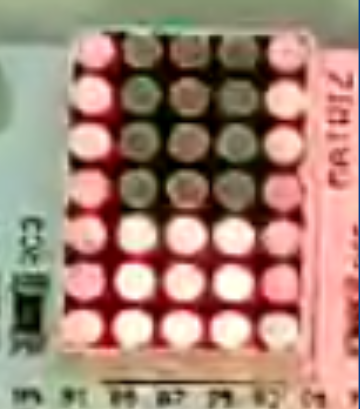
\includegraphics[width=0.3\linewidth]{baixo.png}
    \caption{Nível baixo na matriz de LEDs}
    \label{fig:baixo}
\end{figure}

\begin{figure} [H]
    \centering
    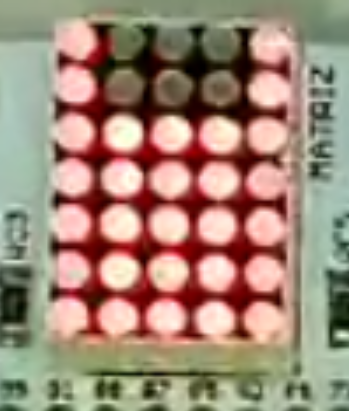
\includegraphics[width=0.3\linewidth]{meio.png}
    \caption{Nível médio na matriz de LEDs}
    \label{fig:meio}
\end{figure}

\begin{figure} [H]
    \centering
    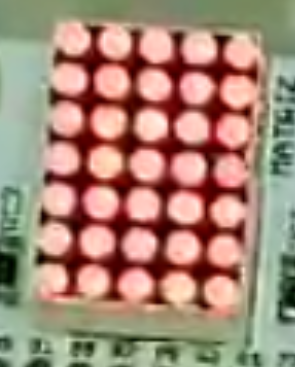
\includegraphics[width=0.3\linewidth]{alto.png}
    \caption{Nível alto na matriz de LEDs}
    \label{fig:alto}
\end{figure}

\begin{figure} [H]
    \centering
    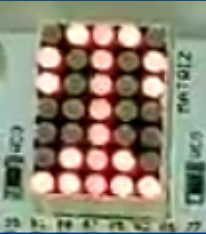
\includegraphics[width=0.3\linewidth]{asp.png}
    \caption{Aspersão representada na matriz de LEDs}
    \label{fig:asp}
\end{figure}

\begin{figure} [H]
    \centering
    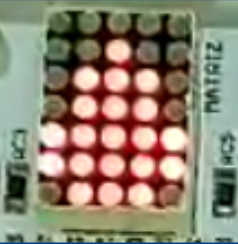
\includegraphics[width=0.3\linewidth]{got.png}
    \caption{Gotejamento representada na matriz de LEDs}
    \label{fig:got}
\end{figure}


Além disso, o estado da válvula de enchimento da caixa d'água é exibido no primeiro dígito (da esquerda para a direita) de um display de 7 segmentos. Neste contexto, a letra "A" indica que a válvula está "Aberta" e a letra "F" que está "Fechada". As figuras pertinentes mostram essas indicações. Adicionalmente, o display de 7 segmentos também exibe o temporizador, que é configurado para iniciar com 30 minutos no modo de Gotejamento e 15 minutos no modo de Aspersão, conforme ilustrado nas Figuras \ref{fig:valv-aberta} e \ref{fig:valv-fechada}.

\begin{figure} [H]
    \centering
    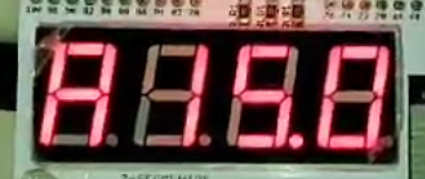
\includegraphics[width=0.4\linewidth]{valv-aberta.png}
    \caption{Válvula aberta e temporizador}
    \label{fig:valv-aberta}
\end{figure}

\begin{figure} [H]
    \centering
    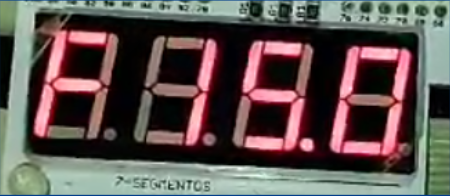
\includegraphics[width=0.4\linewidth]{valv-fechada.png}
    \caption{Válvula fechada e temporizador}
    \label{fig:valv-fechada}
\end{figure}

Em caso de conflito nos sensores, o display de 7 segmentos é capaz de mostrar uma mensagem de erro, alertando sobre a anomalia detectada. Esta funcionalidade é útil para a identificação e resolução rápida de problemas operacionais. A Figura \ref{fig:erro} demonstra a visualização dessa mensagem de erro.

\begin{figure} [H]
    \centering
    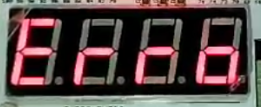
\includegraphics[width=0.4\linewidth]{erro.png}
    \caption{Mensagem de erro}
    \label{fig:erro}
\end{figure}

% --


% Finaliza a parte no bookmark do PDF, para que se inicie o bookmark na raiz
\bookmarksetup{startatroot}% 

% Conclusão
\section*{Considerações finais}
\addcontentsline{toc}{section}{Considerações finais}

Durante o desenvolvimento do projeto, foram enfrentadas diversas dificuldades técnicas significativas. Algumas das principais envolveram a implementação dos \textit{flip-flops}, componentes críticos para o controle de estados e temporização dentro do circuito. Outra complexidade técnica foi a implementação da funcionalidade de parada do temporizador ao atingir o valor zero, garantindo que ele cessasse corretamente suas operações.

O temporizador em si apresentou desafios adicionais, exigindo uma abordagem dedicada para assegurar seu funcionamento conforme especificado. A resolução desses problemas demandou um estudo aprofundado da literatura especializada, além de consultas contínuas com monitores e professores, cujas orientações foram fundamentais para superar as dificuldades encontradas.

Cada módulo do projeto, desde aqueles responsáveis pela matriz de LEDs até os relacionados ao temporizador, foi desenvolvido com o objetivo de atender aos requisitos especificados para o circuito. A matriz de LEDs, por exemplo, foi projetada para alternar periodicamente entre a indicação do nível da caixa d'água e o tipo de irrigação, garantindo uma representação clara das informações.

Os resultados obtidos com esses módulos indicam um desempenho satisfatório em todas as métricas avaliadas, comprovando o êxito do design e da implementação. A integração harmoniosa dos diferentes componentes demonstra a robustez do circuito desenvolvido e sua capacidade de operar dentro dos parâmetros projetados, atendendo às necessidades específicas do sistema de irrigação automatizado.



% --

% \lipsum[1]

% % \begin{citacao}
% % \lipsum[2]
% % \end{citacao}

% \lipsum[3]

% ----------------------------------------------------------
% ELEMENTOS PÓS-TEXTUAIS
% ----------------------------------------------------------
\postextual

% ---
% Título e resumo em língua estrangeira
% ---

% \twocolumn[    		% INICIO DE ARTIGO EM DUAS COLUNAS

% titulo em inglês
\titulo{Problem 2: ... Automated Irrigation (Improvements)!}
\emptythanks
\maketitle

% resumo em português
\renewcommand{\resumoname}{Abstract}
\begin{resumoumacoluna}
 \begin{otherlanguage*}{english}
   This study presents the evolution of an automated irrigation system, initially proposed, with the implementation of an enhanced circuit. The new design incorporates advanced functionalities, including a timer and an improved interface for displaying system information. The development tools Verilog and Quartus were employed for the implementation on the CPLD MAX II board. The results demonstrate the effectiveness of using resources such as synchronous and asynchronous counters, flip-flops, latches, and clock manipulation, highlighting the system's potential to optimize irrigation processes.

   \vspace{\onelineskip}
 
   \noindent
   \textbf{Key-words}: automated irrigation. digital circuits. Verilog. Quartus. CPLD MAX II. digital systems. synchronous counters. asynchronous counters. flip-flops. latches. clock manipulation. agricultural automation. process optimization.






 \end{otherlanguage*}  
\end{resumoumacoluna}

% ]  				% FIM DE ARTIGO EM DUAS COLUNAS
% ---

% ----------------------------------------------------------
% Referências bibliográficas
% ----------------------------------------------------------
\bibliography{abntex2-modelo-references}

\end{document}
